
After the freeze-out of the Dark Matter (DM) in the early Universe, the annihilation continuous to today but in smaller rate, principally in regions where the concentration of DM is high, like the center of our Galaxy.
Therefore, exits the possibility to see this annihilations looking for in the flux that reach the earth and in that way check the freeze-out mechanism. However to measure the expected flux after DM annihilation is so challenging because It is typically much smaller than the background flux generated for Astrophysical processes.

One strategy to identify DM signals is to search for gamma ray spectral features as gamma ray lines.
In the case of the Milky Way center, DM particles are expected to be very non-relativistic, $v\approx 10^{-3}$, thus generating monoenergety photons in the annihilation process. They are qualitatively very different from the ones expected from the known astrophysical background and for that reason a good form to find the DM in the Universe.
Search for gamma ray spectral features provide limits on the model parameter space and sometimes are competitive with direct detection.  

In the particular case of the SDFDM model with real scalars singlets we can have scalar or fermionic DM like we described in the Sec.~\ref{sec:model-with-scalars}. The goal of this chapter is to describe the spectral features generated in this two cases.





%%%%%%%%%%%%%%%%%%%%%%%%%%%%%%%%%%%%%%%%%%%%%%%%%%%%%%%%%%%%%%%%%%%%%%%%%%%%%%%%%%%%%%%%%%%%%%%%%
\section{DM annihilation into $\gamma\gamma$ and $\gamma Z$}

\subsection{Four-momentum for DM annihilation into $\gamma\gamma$ and $\gamma Z$}

\begin{figure}[h]
\begin{center}
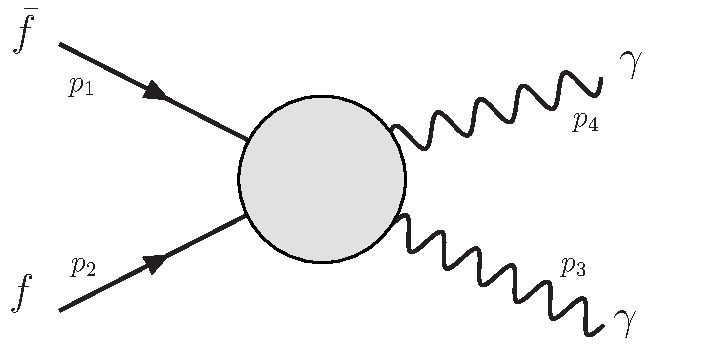
\includegraphics[scale=0.45]{annihilation_in_gammagamma}
\end{center}
\caption{General annihilation into two photons.}
\label{fig:annihilationgg}
\end{figure}

In the s-wave approximation we consider an initial state of two particles (fermions or scalars) non-relativistic with a initial relative velocity going to zero. In this case, we have an initial state with orbital angular momentum $L=0$ and spin $S=0$. The momentum shown in the Fig.~\eqref{fig:annihilationgg} for the case of fermions annihilation process in the CM frame are approximately given by
\begin{align}
p_{1}=&(E,m\vec{v})\approx(m,0,0,0)\nonumber\\
p_{2}=&(E,-m\vec{v})\approx(m,0,0,0)\nonumber\\
p_{3}=&(E_{\gamma},0,0,E_{\gamma})\nonumber\\
p_{4}=&(E_{\gamma},0,0,-E_{\gamma})\,.
\end{align}
%
Therefore, in this limit, the Mandelstan variables are
\begin{align*}
s=&(p_1+p_2)^2=4E^2=4m^2(1+v^2)=4m^2\left(1+\dfrac{v_r^2}{4}\right)=4m^2(1+\epsilon)\\
t=&(p_1-p_3)^2=p_1^2+p_3^2-2p_1p_3\approx m^2-2mE_{\gamma}\\
u=&(p_1-p_4)^2=p_1^2+p_4^2-2p_1p_4\approx m^2-2mE_{\gamma}\,,
\end{align*}
where $v_r=\sqrt{4\epsilon}$ is the relative velocity of the two initial particles in the CM frame.
Now, using the known relation $s+t+u=\sum_im_i^2=2m^2$ and the last equation, we get that $E_{\gamma}\approx m$ and therefore we get the next approximate relation for the Mandelstan variables
\begin{align}
u&\rightarrow t \nonumber\\
t&\rightarrow m^2-\dfrac{s}{2} \nonumber\\
s&\rightarrow 4m^2(1+\epsilon)\,,
\end{align}
where $\epsilon\approx 0$ take into account the non-zero initial velocity of the particles.



\begin{figure}[h]
\begin{center}
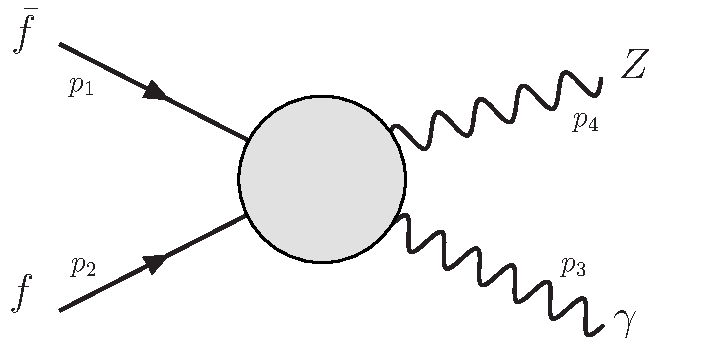
\includegraphics[scale=0.45]{annihilation_in_gammaz}
\end{center}
\caption{General annihilation into one photon and one Z gauge boson.}
\label{fig:annhilation-gz}
\end{figure}
%
In this case of DM annihilation into $\gamma Z$, the momentums shown in the Fig.~\eqref{fig:annhilation-gz} in the s-wave limit are
\begin{align}
p_1=&(E,m\vec{v})\approx(m,0,0,0)\nonumber\\
p_2=&(E,-m\vec{v})\approx(m,0,0,0)\nonumber\\
p_3=&(E_{\gamma},0,0,E_{\gamma})\nonumber\\
p_4=&(E_{Z},0,0,-|\vec{p}_{Z}|=-E_{\gamma})\,.
\end{align}
Using the conservation of the energy and the momentum we have
\begin{align}
E_{\gamma}=&m-\dfrac{m_{Z}^2}{4m}\nonumber\\
E_{Z}=&2m-E_{\gamma}\,.
\end{align}
%
The Mandelstan variables for this process are
\begin{align}
s=&(p_1+p_2)^2=p_1^2+p_2^2+2p_1p_2 = 4m^2(1+\epsilon)\nonumber\\
t=&(p_1-p_3)^2=p_1^2+p_3^2-2p_1p_3\approx m^2-2mE_{\gamma}=-m^2+\dfrac{m_Z^2}{2}\nonumber\\
u=&(p_1-p_4)^2=p_1^2+p_4^2-2p_1p_4\approx m^2+m_{Z}^2-2mE_{Z}=-m^2+\dfrac{m_Z^2}{2}\,.
\end{align}
%
Thus, using the equation $s+t+u=\sum_im_i^2=2m^2+m_Z^2$, we get the next relation 
\begin{align}
u&\rightarrow t \nonumber\\
t&\rightarrow m^2+\dfrac{m_Z^2}{2}-\dfrac{s}{2} \nonumber\\
s&\rightarrow 4m^2(1+\epsilon)\,,
\end{align}
where $\epsilon\approx 0$ take into account the non-zero initial velocity of the particles.







%%%%%%%%%%%%%%%%%%%%%%%%%%%%%%%%%%%%%%%%%%%%%%%%%%%%%%%%%%%%%%%%%%%%%%%%%%%%%%%%%%%%%%%%%%%%%%%%%%%%%%%%%%%%
\section{Gamma-ray lines spectral features from scalar DM}

\begin{figure}
\centering
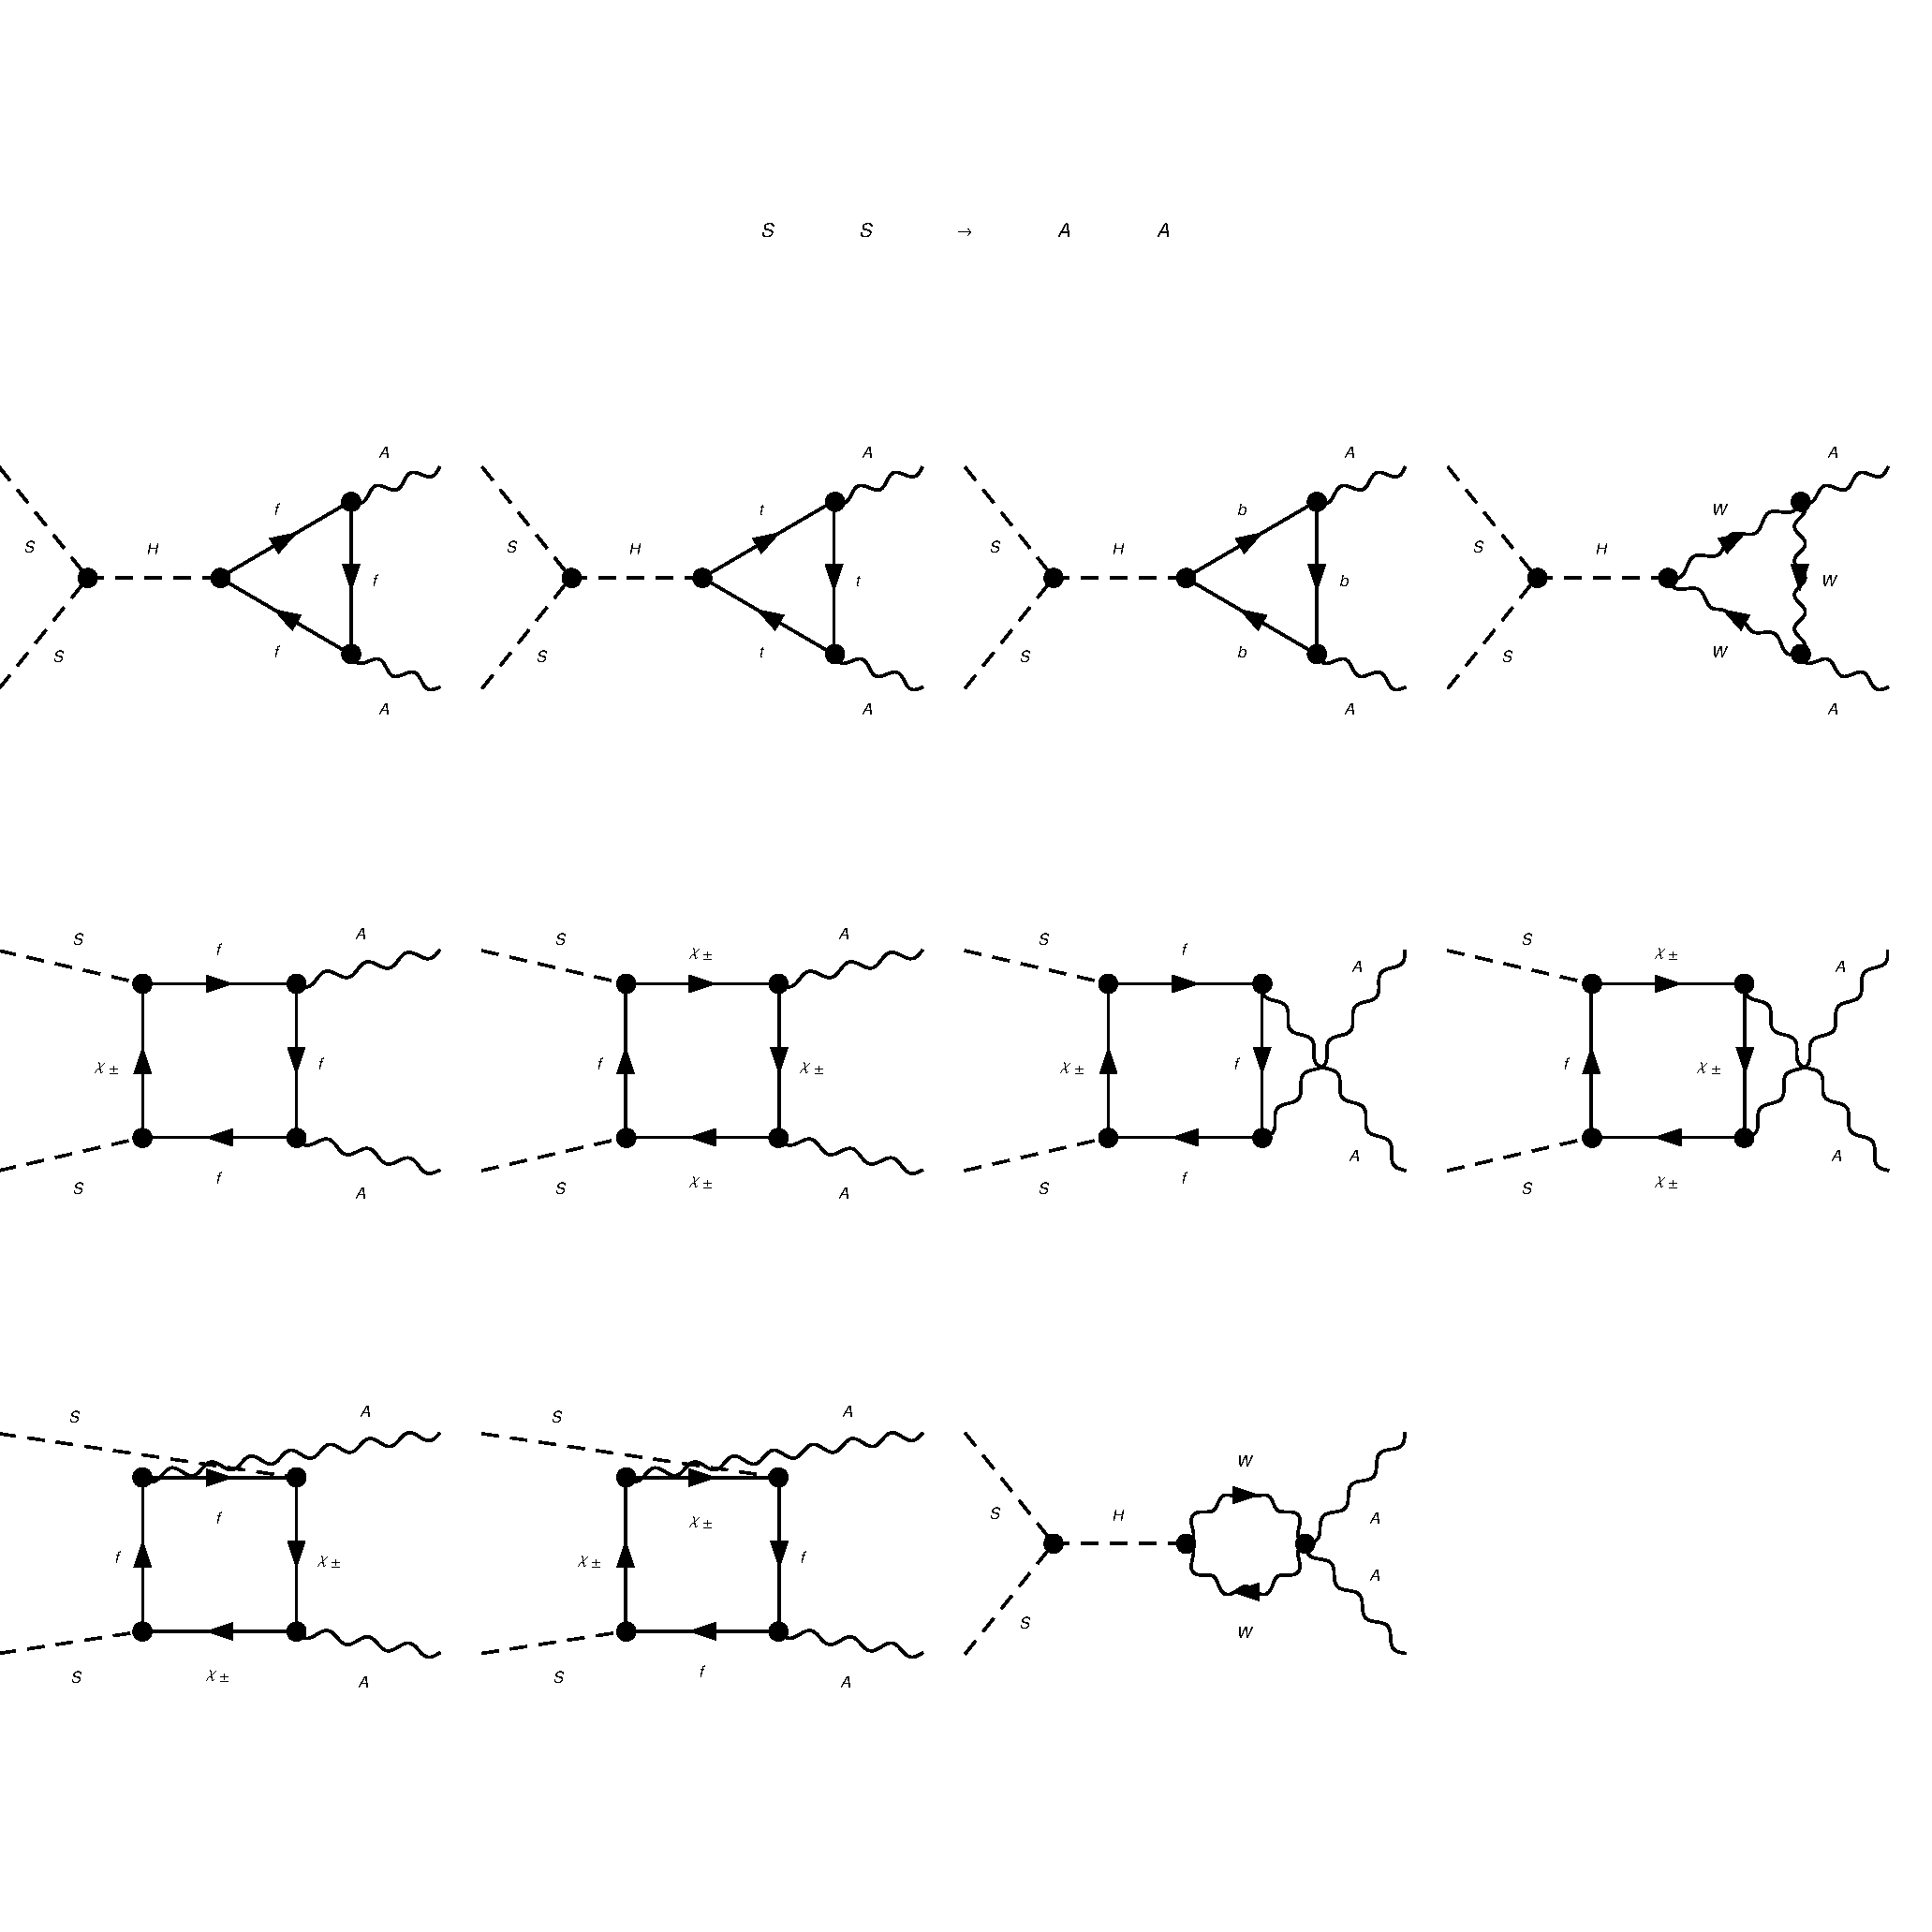
\includegraphics[scale=0.52]{T13A-scalar-to-GG-diagrams}
\caption{Feynman diagrams for $S S \to\gamma\gamma$ generated with \textsc{FeynArts}~\cite{Hahn:2000kx}. The diagrams generating the annihilation into $\gamma Z$ can be obtained by replacing one $\gamma$ in the final state by a Z-boson. In order to be more readable we show the diagrams in the unitary gauge. We only used the third family of quarks and one lepton family $f$.  We don't show the equivalent topologies with crossed initial or final state legs.}
\label{fig:scalar-to-GG}
\end{figure}

In general, the DM annihilation into $\gamma\gamma$ and $\gamma Z$ are processes generated at one loop level. They are so complicated and we have to use some computational tools that we will describe latter and use some analytical fats as the gauge and the $CP$ symmetry invariance.

In general, we used the Feynman gauge which is mandatory for the implementation in \textsc{FormCalc}~\cite{Hahn:1998yk} via \textsc{FeynRules}~\cite{Christensen:2008py}. In the Fig.~\ref{fig:scalar-to-GG} we show the Feynman diagrams for DM annihilation into $\gamma\gamma$ generated with \textsc{FeynArts}~\cite{Hahn:2000kx}. The diagrams for the annihilation into $\gamma Z$ are the same. They can be obtained by replacing one photon in the final state by the Z boson. In order to be more readable we show the diagrams in the unitary gauge. We only used the third family of quarks and one lepton family $f$.  We don't show the equivalent topologies with crossed initial or final state legs.

\subsection{Amplitude for scalar DM annihilation}

In general, it can be shown that the amplitude for scalar DM annihilation into $\gamma\gamma$ can be cast as
%
\begin{align}
\mathcal{M_{\gamma\gamma}}=&(\mathcal{M_{\gamma\gamma}})^{\mu\nu}\epsilon_{\mu}^*(p_3)\epsilon_{\nu}^*(p_4)
=\mathcal{A}_{\gamma\gamma}\left(g^{\mu\nu}-\dfrac{p_4^{\mu}p_3^{\nu}}{2m^2}\right)\epsilon_{\mu}^*(p_3)\epsilon_{\nu}^*(p_4)\,,
\end{align} 
%
where, $\mathcal{A}_{\gamma\gamma}$ is an scalar function (form factor), $\epsilon^*(p_3)_{\mu}$ and $\epsilon^*(p_4)_{\nu}$ are the polarization vectors of the photons and $m$ is the DM mass. Note that $\mathcal{M}^{\mu\nu}$ satisfied the Ward identity
$p_{3\mu}\mathcal{M}^{\mu\nu}=p_{4\nu}\mathcal{M}^{\mu\nu}=0\,$.
Even more, in the limit of zero relative velocity it can be shown that
%
\begin{align}
\label{eq:M-scalar-GG}
\mathcal{M_{\gamma\gamma}}=\mathcal{A}_{\gamma\gamma}\,g^{\mu\nu}\epsilon_{\mu}^*(p_3)\epsilon_{\nu}^*(p_4)\,.
\end{align}

On the other hand, the amplitude for annihilation into $\gamma Z$ can be cast, in the zero velocity limit, as
\begin{align}
\label{eq:M-scalar-GZ}
\mathcal{M}_{\gamma Z}=\mathcal{A}_{\gamma Z}\,g^{\mu\nu}\epsilon_{\mu}^*(p_3)\epsilon_{\nu}^*(p_4)\,,
\end{align} 
%
where $\mathcal{A}_{\gamma Z}$ is the corresponding form factor. 
As you can see, it is almost equal to the Eq.~\eqref{eq:M-scalar-GG} with the corresponding form factor. 


Now, we use the programs \textsc{FeynArts}~\cite{Hahn:2000kx} and \textsc{FormCalc}~\cite{Hahn:1998yk} to compute the amplitudes $\mathcal{M}_{\gamma\gamma}$ and $\mathcal{M}_{\gamma Z}$. In general, when \textsc{FeynArts} and \textsc{FormCalc} compute the amplitude we get an big expression that in general depend of the Passarino Veltman one loop integrals that we describe in the Appendix~\ref{sec:passarino-veltman}. Numerically we can evaluated this expression using \textsc{LoopTools}~\cite{Hahn:1998yk}. However, our goal is to get an analytical result and for that reason we implement an algorithm that we describe in the Appendix~\ref{sec:CD-reduction} in order to reduce the Passarino Veltman integrals in the \textsc{FormCalc} output. The algorithm reduce the fourth-point function to three point functions and all the coefficients tensor of the loop integrals. Usually, the results are given in terms of the scalar Passarino Veltman $C_0$ which can be given in terms of the dilogarithm Li$_{2}$ functions. In this case, the notation is more compact and readable.

The form factor obtained are:
\begin{align}
\label{eq:form-factor-SSGG}
\mathcal{A}_{\gamma\gamma}=\mathcal{A}^{h_i}_{\gamma\gamma} + \mathcal{A}^{\lambda_{SH}}_{\gamma\gamma}
\end{align}
%
\begin{align}
\mathcal{A}^{h_i}_{\gamma\gamma}
=&-\dfrac{\alpha\, h_{i}^2}{\pi} \Bigg{\{ } 2+m^2 \Big{[}
 \dfrac{1-\mu+\epsilon}{1+\mu-\epsilon}\dfrac{2\epsilon}{\mu-\epsilon}C_0(-m^2,m^2,0;m_{fi}^2,M_D^2,m_{fi}^2)\nonumber \\
+&\dfrac{1-\mu-\epsilon}{1-\mu+\epsilon}\dfrac{2\mu}{\epsilon-\mu}C_0(-m^2,m^2,0;M_D^2,m_{fi}^2,M_D^2)
+\dfrac{4\epsilon(1-\epsilon)}{1+\mu-\epsilon}C_0(4m^2,0,0;m_{fi}^2,m_{fi}^2,m_{fi}^2)\nonumber \\
+&\dfrac{4\mu(1-\mu)}{1+\epsilon-\mu}C_0(4m^2,0,0;M_D^2,M_D^2,M_D^2) \Big{] } \Bigg{\} } 
\end{align}
%

\begin{align}
\mathcal{A}^{\lambda_{SH}}_{\gamma\gamma}
=&\dfrac{\alpha}{\pi}\lambda^{SH} \bigg(\dfrac{12 m^2 + 3 m_h^2 + 16 m_t^2 + 18 m_W^2}{3(4 m^2 -  m_h^2)} +\dfrac{32 (m^2 - m_t^2) m_t^2}{3 (-4 m^2 + m_h^2)}C_0(4m^2,0,0;m_t^2,m_t^2,m_t^2)\\
&+\dfrac{m_W^2 (-24 m^2 + m_h^2 + 12 m_W^2)}{(4 m^2 - m_h^2)}C_0(4m^2,0,0;m_W^2,m_W^2,m_W^2) \bigg)\,,
\end{align}
%
where $\epsilon = m_{fi}^2/m^2$ and $\mu = M_D^2/m^2$.
$C_0$ is the scalar three-point Passarino-Veltman integral~\cite{Passarino:1978jh}. \\
Note that wee split the amplitude in two gauge invariant parts; $\mathcal{A}^{h_i}_{\gamma\gamma}$ which only depend of the coupling $h_{i}$ of the Lagrangian~\eqref{eq:lt13a} and generated the boxes diagrams shown in the Fig.~\ref{fig:scalar-to-GG}. This amplitude were computed and analyzed in~\cite{Ibarra:2014qma}, for that reason we didn't do an detailed analysis of this case, it only help us to check that our algorithm of the loop integrals is working properly. 
The other contribution $\mathcal{A}^{\lambda_{SH}}_{\gamma\gamma}$ seems to be less important because $\lambda^{SH}$ needs to be small~\cite{Ibarra:2014qma} according to direct detection's experiments (LUX and XENON1T).


%\begin{widetext}
\begin{eqnarray}
\label{eq:form-factor-SSGZ}
\mathcal{A}_{\gamma Z}\!\!&\,=\,&\!\!
-\dfrac{\alpha\, h_{i}^2 \tan\theta_W}{\pi} \Bigg{\{ } 
2-\frac{\xi}{4-\xi}B_0\left(m_Z^2;m_{fi}^2,m_{fi}^2\right)
-\frac{\xi}{4-\xi}B_0\left(m_Z^2;M_D^2,M_D^2\right)\nonumber\\
&&
+\frac{2\xi\left(1+\mu+\epsilon\right)}
{\left(4-\xi\right)\left(1+\mu-\epsilon\right)\left(1+\epsilon-\mu\right)}
\left[1-\frac{1-\mu+\epsilon}{1+\mu+\epsilon}\frac{\epsilon}{2}\right]
B_0\left(m^2;m_{fi}^2,M_D^2\right)\nonumber\\
&&
-\frac{\epsilon}{1+\mu-\epsilon}\frac{\xi}{4-\xi}
B_0\left(4m^2;m_{fi}^2,m_{fi}^2\right)
-\frac{2\mu}{1+\epsilon-\mu}\frac{\xi}{4-\xi}
B_0\left(4m^2;M_D^2,M_D^2\right)\nonumber\\
&&
+m_\chi^2\left\{
\frac{\epsilon}{2}\frac{4-4\epsilon-\xi}{1+\mu-\epsilon}
C_0\left(m_Z^2,4m^2,0;m_{fi}^2,m_{fi}^2,m_{fi}^2\right)
+\mu\frac{4-4\mu-\xi}{1+\epsilon-\mu}
C_0\left(m_Z^2,4m^2,0;M_D^2,M_D^2,M_D^2\right)\right.\nonumber\\
&&
+\frac{\epsilon}{2}\left[\frac{\left(4+\xi\right)\left(-2+2\mu+2\epsilon+\xi\right)}
{\left(1+\mu-\epsilon\right)\left(4\epsilon-4\mu+\xi\right)}
+\frac{1}{2}\frac{4-4\epsilon-\xi}{1+\mu-\epsilon}
\right]
C_0\left(-m^2+\frac{m_Z^2}{2},m^2,0;m_{fi}^2,M_D^2,m_f^2\right)\nonumber\\
&&
+\frac{\mu}{2}\left[\frac{\left(4+\xi\right)\left(-2+2\epsilon+2\mu+\xi\right)}
{\left(1+\epsilon-\mu\right)\left(4\mu-4\epsilon+\xi\right)}
-\frac{8\epsilon}{4\mu-4\epsilon+\xi}
\right]
C_0\left(-m^2+\frac{m_Z^2}{2},m^2,0;M_D^2,m_{fi}^2,M_D^2\right)\nonumber\\
&&
+\left[
\frac{2\xi\left(1+\mu\right)+\epsilon\left(4\mu-\xi\right)}{4\left(1+\mu-\epsilon\right)}
-\frac{4\left(1+\mu\right)}{4-\xi}+\frac{4\mu\left(1+\mu-2\epsilon\right)}{4\mu-4\epsilon+\xi}
\right]C_0\left(-m^2+\frac{m_Z^2}{2},m^2,m_Z^2;m_{fi}^2,M_D^2,m_{fi}^2\right)\nonumber\\
&&
+\left[
\frac{2\mu\left(1-\mu+3\epsilon\right)+\xi\left(1+\epsilon\right)}
{2\left(1+\epsilon-\mu\right)}
-\frac{4\left(1+\mu+\epsilon\right)}{4-\xi}
+\frac{4\epsilon\left(1+3\mu+\epsilon\right)}{4\epsilon-4\mu+\xi} \right]\nonumber \\
&&
\left. C_0\left(-m^2+\frac{m_Z^2}{2},m^2,m_Z^2;M_D^2,m_{fi}^2,M_D^2\right)
\right\} \Bigg{\} } \,,
\end{eqnarray}
%\end{widetext}
where $\xi=m_Z^2/m^2$ and $B_0$ is the Passarino Veltaman two-point function defined in the Appendix~\ref{sec:passarino-veltman}.
%\begin{equation}
%B_0\left(p_1^2;m_1^2,m_2^2\right)=
%\int\frac{d^d\ell}{i\pi^2}
%\frac{1}{\ell^2-m_1^2}\frac{1}{\left(\ell+p_1\right)^2-m_2^2}\,.
%\end{equation}



%%%%%%%%%%%%%%%%%%%%%%%%%%%%%%%%%%%%%%%%%%%%%%%%%%%%%%%%%%%%%%%%%%%%%%%%%%%%%%%%%%%%%%%%%%%%%%%%%%%%%
\subsection{Velocity averaged annihilation cross section $\langle \sigma v \rangle$ for scalar DM annihilation into $\gamma\gamma$ and $\gamma Z$}

In the the Appendix~\ref{sec:sigmav} we compute the thermal velocity averaged annihilation cross section for each process.
For the case of DM annihilation into two photons~Fig.\ref{fig:annihilationgg}, $\chi^0\chi^0\rightarrow\gamma\gamma$: $m_1=m_2=m$, $m_3=m_4=0$, it is given by
%
\begin{align}
\langle\sigma v_r\rangle=&\dfrac{1}{32\pi\, m^2}\overline{{|\mathcal{M}_{\gamma\gamma}|^2}}\left(1-\dfrac{v_r^2}{8}+\mathcal{O}(v_r^4)\right)\,.
\end{align}
Thus, using the Eq.~\eqref{eq:M-scalar-GG}, the s-wave contribution is
\begin{align}
\langle\sigma v_r\rangle\Big{\vert}_{\text{s-wave}}
=&\dfrac{1}{32\pi\, m^2}\overline{{|\mathcal{M}_{\gamma\gamma}|^2}}
=\dfrac{1}{32\pi\, m^2}\dfrac{1}{2}\sum_{r_3r_4=\pm 1}{|\mathcal{M}_{\gamma\gamma}|^2}
=\dfrac{1}{32\pi\, m^2}\dfrac{1}{2}\sum_{r_3r_4=\pm 1} |\mathcal{A}_{\gamma\gamma}\,g^{\mu\nu}\epsilon_{\mu}^*(p_3,r_3)\epsilon_{\nu}^*(p_4,r_4)|^2\nonumber \\
=&\dfrac{1}{32\pi\, m^2} |\mathcal{A}_{\gamma\gamma}|^2 \,,
\end{align}
%
where $r_{3,4}$ are the polarization of final states and the form factor $\mathcal{A}_{\gamma\gamma}$ is given by Eq.~\ref{eq:form-factor-SSGG}.

For the case of DM annihilation into one photon and one $Z$ gauge boson~Fig.\ref{fig:annhilation-gz}, $\chi^0\chi^0\rightarrow\gamma Z$: $m_1=m_2=m$, $m_3=0$ and $m_4=m_Z$, it is given by
%
\begin{align}
\langle\sigma v_r\rangle
= &  \dfrac{1}{32\pi\, m^2}\left[ 1- \left(\dfrac{m_Z}{2m}\right)^2 +\dfrac{1}{8}\left(-1+3\left(\dfrac{m_Z}{2m}\right)^2\right) v_r^2 + \mathcal{O}(v_r^4)\right]\overline{{|\mathcal{M}_{\gamma Z}|^2}} \,.
\end{align}
%
Thus,  using the Eq.~\eqref{eq:M-scalar-GZ}, the s-wave contribution is
\begin{align}
\langle\sigma v_r\rangle\Big{\vert}_{\text{s-wave}}
= & \dfrac{1}{32\pi\, m^2}\left( 1- \dfrac{m_Z^2}{4m^2} \right)\overline{{|\mathcal{M}_{\gamma Z}|^2}} 
=\dfrac{1}{32\pi\, m^2}\left( 1- \dfrac{m_Z^2}{4m^2} \right)\sum_{r_3r_4=\pm 1}{|\mathcal{M}_{\gamma Z}|^2}\nonumber \\
=&\dfrac{1}{32\pi\, m^2}\left( 1- \dfrac{m_Z^2}{4m^2} \right)\sum_{r_3r_4=\pm 1} |\mathcal{A}_{\gamma Z}\,g^{\mu\nu}\epsilon_{\mu}^*(p_3,r_3)\epsilon_{\nu}^*(p_4,r_4)|^2
=\dfrac{1}{16\pi\, m^2}\left( 1- \dfrac{m_Z^2}{4m^2} \right) |\mathcal{A}_{\gamma Z}|^2\,,
\end{align}
where $r_{3,4}$ are the polarization of final states and the form factor $\mathcal{A}_{\gamma Z}$ is given by Eq.~\ref{eq:form-factor-SSGZ}.
%








%%%%%%%%%%%%%%%%%%%%%%%%%%%%%%%%%%%%%%%%%%%%%%%%%%%%%%%%%%%%%%%%%%%%%%%%%%%%%%%%%%%%%%%%%%%%%%%%%%%%%%%%%%%%
\section{Gamma-ray lines spectral features from fermion DM}

The DM anniquilation into $\gamma\gamma$ and $\gamma Z$ are generated at one loop level. In general, for the processes $\chi^0\chi^0\to\gamma\gamma$ and $\chi^0\chi^0\to\gamma Z$ there are 148 and 220 diagrams respectively in the Feynman gauge which is mandatory for the implementation in \textsc{FormCalc}~\cite{Hahn:1998yk} via \textsc{FeynRules}~\cite{Christensen:2008py}. In the Fig.~\ref{fig:2F-to-GG} and Fig.~\ref{fig:2F-to-GZ} of the Appendix~\ref{sec:xxtogz} we show the diagrams for the unitary gauge in order to be more readable.  We only used the third family for the quarks and SM lepton and  we don't show the equivalent topologies with crossed initial or final state legs.

%
\begin{figure}
\centering
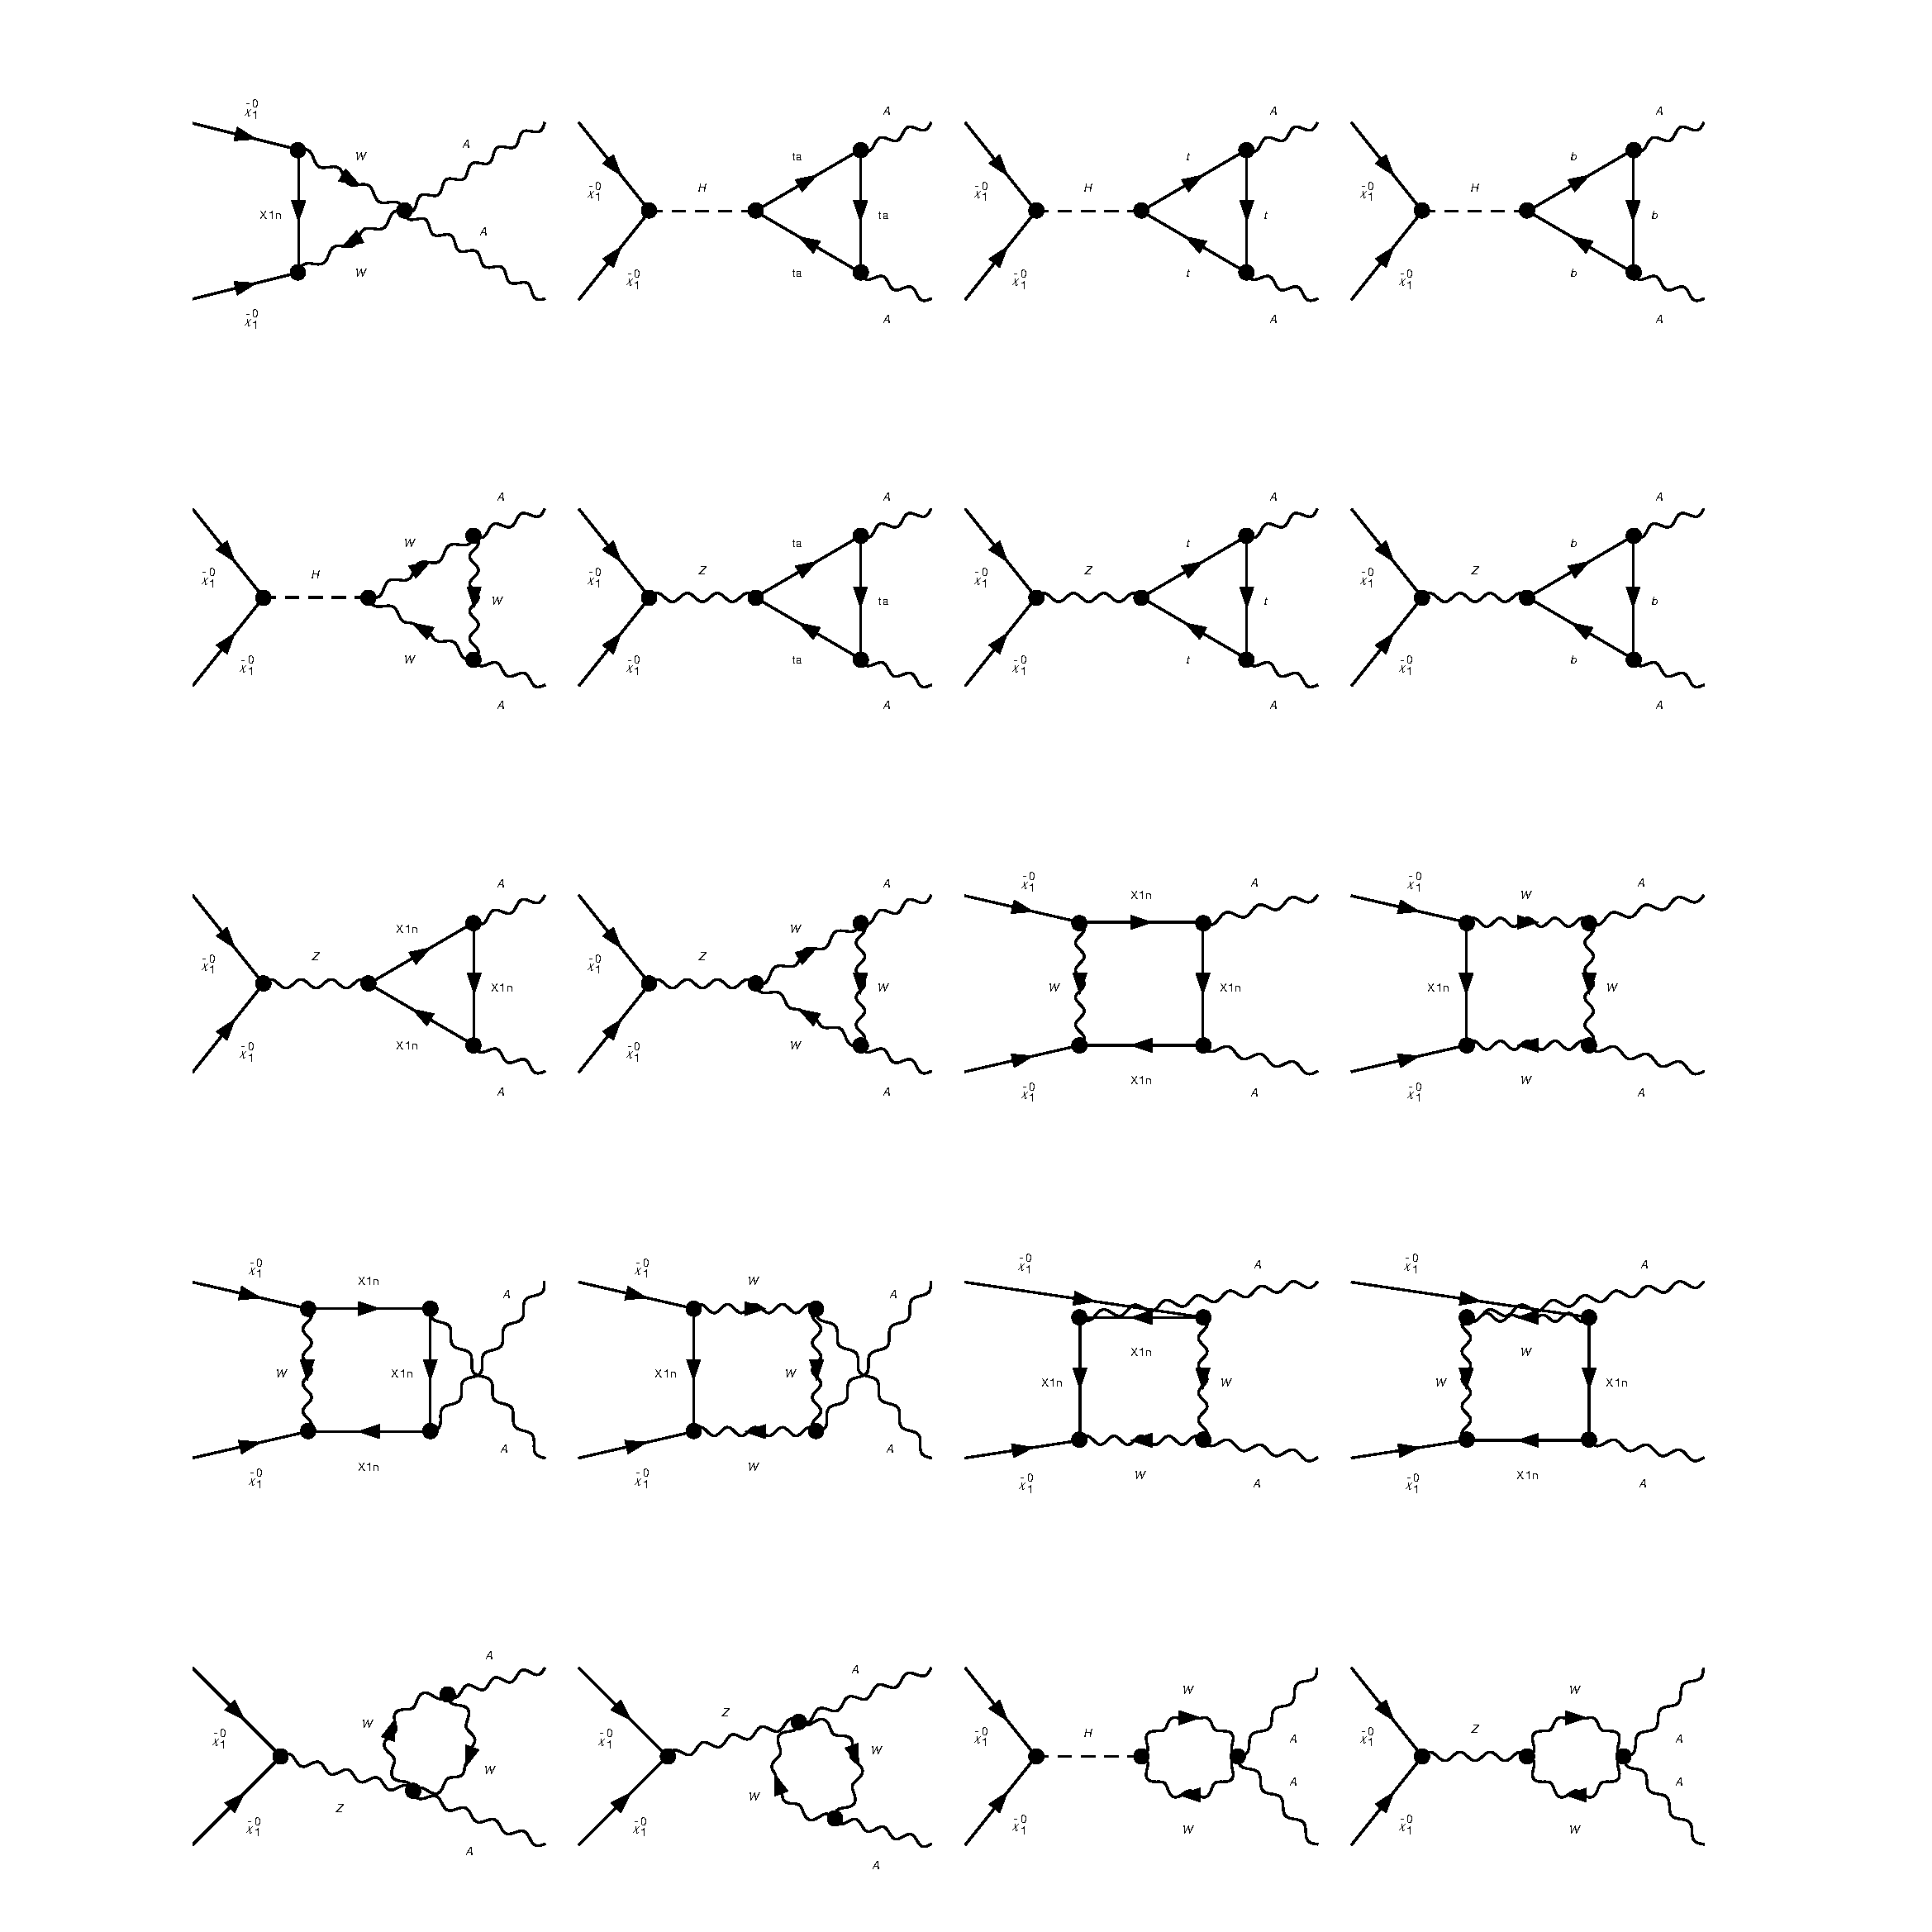
\includegraphics[scale=0.52]{2F-2g-diagrams}
\caption{Feynman diagrams for $\chi^0\chi^0 \to\gamma\gamma$ generated with \textsc{FeynArts}~\cite{Hahn:2000kx}. In order to be more readable we show the diagrams in the unitary gauge. We only used the third family of quarks and one lepton family $\tau= $ ta.  We don't show the equivalent topologies with crossed initial or final state legs.}
\label{fig:2F-to-GG}
\end{figure}
%
%\begin{figure}
%\centering
%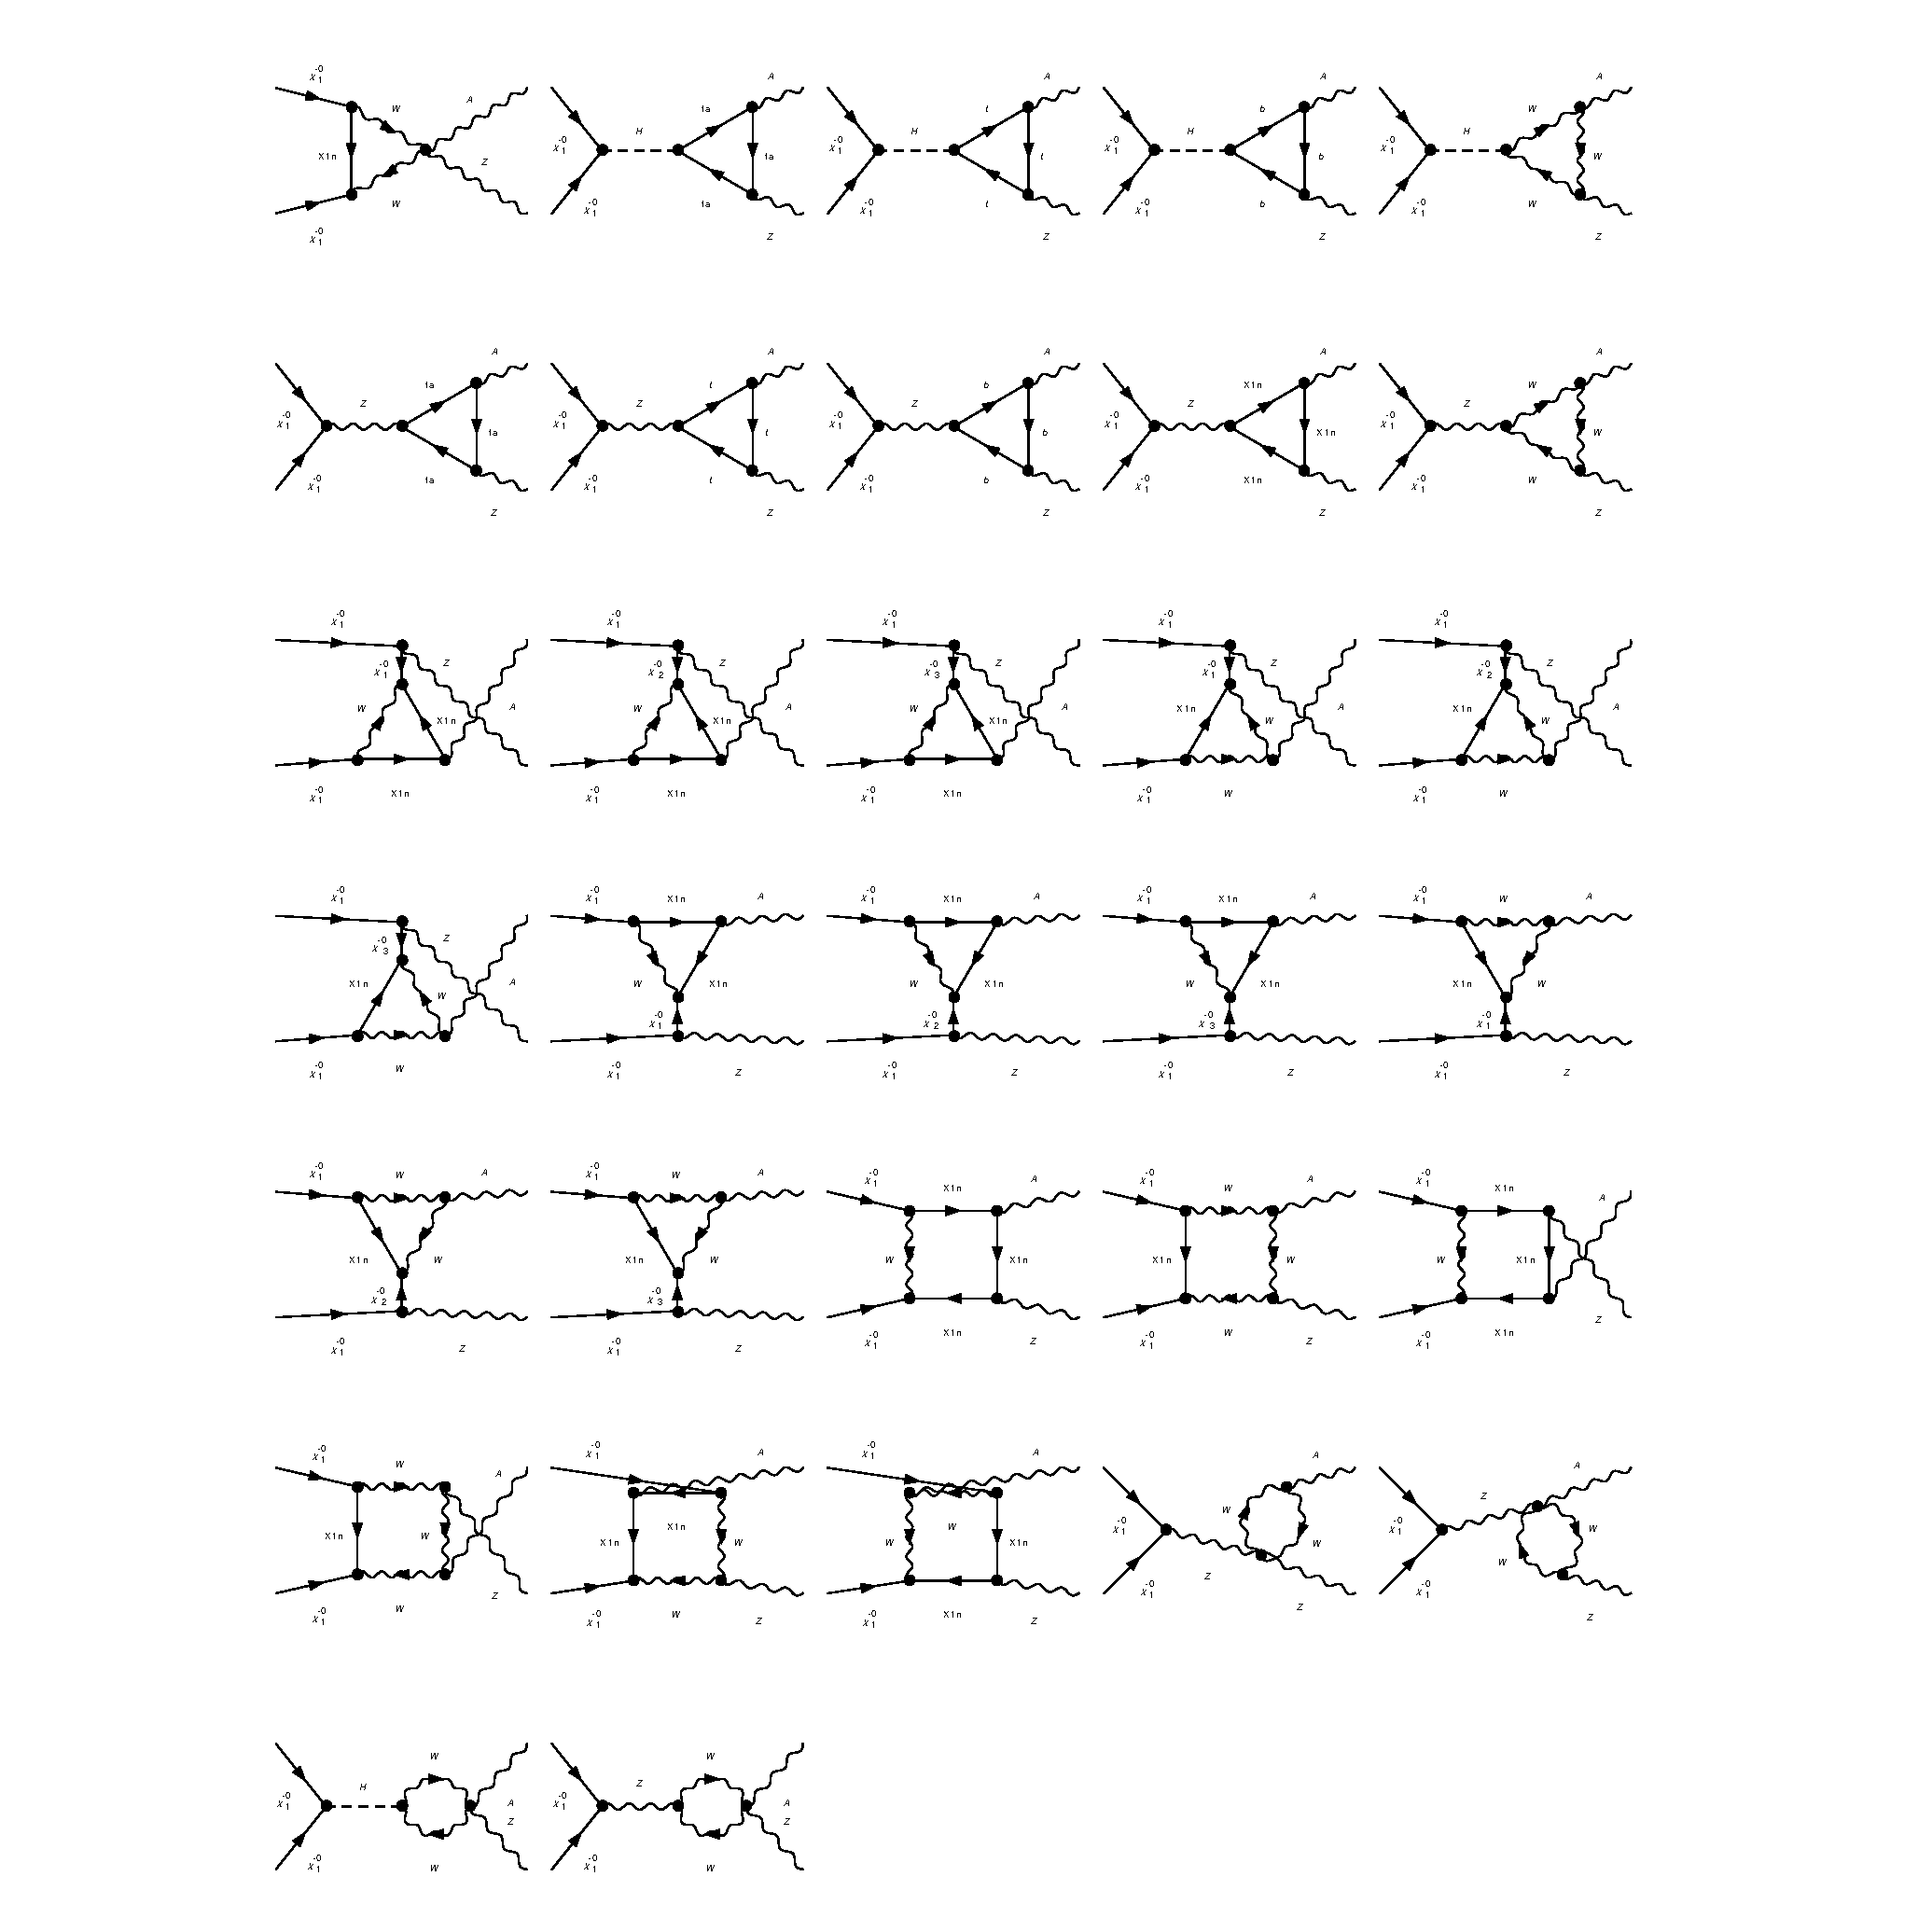
\includegraphics[scale=0.57]{2F-gz-diagrams}
%\caption{Feynman diagrams for $\chi^0\chi^0 \to\gamma Z$ generated with \textsc{FeynArts}~\cite{Hahn:2000kx}. In order to be more readable we show the diagrams in the unitary gauge. We only used the third family of quarks and one lepton family $f$.  We don't show the equivalent topologies with crossed initial or final state legs.}
%\label{fig:2F-to-GZ}
%\end{figure}
%%


%%%%%%%%%%%%%%%%%%%%%%%%%%%%%%%%%%%%%%%%%%%%%%%%%%%%%%%%%
\subsection{Amplitude for fermion DM annihilation}

In the annihilation of the dark matter into two photons show in the Fig.~\ref{fig:annihilationgg}, in general the amplitude is given by
\begin{align}
\label{eq:M1-fermion-GG}
\mathcal{M}_{\gamma\gamma}=\mathcal{M}^{\mu\nu}\epsilon_{\mu}^*(p_3)\epsilon_{\nu}^*(p_4)=\left[\bar{v}_{\sigma 1}\Gamma^{\mu\nu}u_{\sigma 2}\right]\epsilon_{\mu}^*(p_3)\epsilon_{\nu}^*(p_4)\,,
\end{align}
%
where $\Gamma^{\mu\nu}$ comes for the Lorentz structure of the annihilation process, $v_{\sigma 1}$ and $v_{\sigma 2}$ are Dirac spinors for the fermions with spin $\sigma 1,2$ respectively and $\epsilon_{\mu},\epsilon_{\nu}$ are the polarization vectors of the photons. 

In the s-wave limit, the initial state has orbital angular momenta $L=0$ and its wave function $\Psi(p,s)$ must to be antisymmetry because we have two identity fermions in the initial state. Therefore, it must be spin antisymmetry with $S=0$.
%
Considering the wave function $|\Psi_{s=0}\rangle=\tfrac{1}{\sqrt{2}}\left[\uparrow\downarrow|\rangle-|\downarrow\uparrow\rangle\right]$ for the antisymmetry initial state, the amplitude $\mathcal{M^{\mu\nu}}$ in the Eq.~\eqref{eq:M1-fermion-GG} will be given by:
%
\begin{align}
\label{eq:muv}
\mathcal{M}^{\mu\nu}
&=\dfrac{1}{\sqrt{2}}\left[\bar{v}_{\uparrow}\Gamma^{\mu\nu}u_{\downarrow}
-\bar{v}_{\downarrow}\Gamma^{\mu\nu}u_{\uparrow}\right]\nonumber \\
&=\dfrac{1}{\sqrt{2}}\text{Tr}\left[\Gamma^{\mu\nu}u_{\downarrow}\bar{v}_{\uparrow}
-\Gamma^{\mu\nu}u_{\uparrow}\bar{v}_{\downarrow}\right]\,.
\end{align}   
In the last equation we used the properties
\begin{align*}
a^*Mb=\sum_{ij}a_i^*b_j=\sum_{ij}M_{ij}b_ja^*_i=\sum_{ij}M_{ij}(ba^*)_{ji}=\sum_i(Mba^*)_{ii}
=\text{Tr}[Mba^*].
\end{align*}
%
According to the Weyl represestation for the spinors:
\begin{align}
\label{eq:weyl_spinors}
u_{\downarrow}=\sqrt{m}
\begin{pmatrix}
1 \\ 0 \\ 1 \\ 0
\end{pmatrix}\hspace{1 cm}
u_{\uparrow}=\sqrt{m} 
\begin{pmatrix}
0 \\ 1 \\ 0 \\ 1
\end{pmatrix}
\hspace{1.0 cm}
v_{\downarrow}=\sqrt{m}
\begin{pmatrix}
1 \\ 0 \\ -1 \\ 0
\end{pmatrix}\hspace{1 cm}
v_{\uparrow}= -\sqrt{m} 
\begin{pmatrix}
0 \\ 1 \\ 0 \\ -1
\end{pmatrix}\,,
\end{align}
we have
\begin{align}
\mathcal{M}^{\mu\nu}
%=&\tfrac{1}{\sqrt{2}}\text{Tr}\left[\Gamma^{\mu\nu}u_{\downarrow}\bar{v}_{\uparrow}
%-\Gamma^{\mu\nu}u_{\uparrow}\bar{v}_{\downarrow}\right]\nonumber \\
=&\dfrac{m}{\sqrt{2}}\text{Tr}\left[
\Gamma^{\mu\nu}\begin{pmatrix}
0\\1\\0\\1
\end{pmatrix}
(-1)\begin{pmatrix}
0&1&0&-1
\end{pmatrix}\gamma^0 -
\Gamma^{\mu\nu}\begin{pmatrix}
1\\0\\1\\0
\end{pmatrix}
\begin{pmatrix}
1&0&-1&0
\end{pmatrix}\gamma^0
\right] \nonumber\\
=&-\dfrac{m}{\sqrt{2}}\text{Tr}\left[
\Gamma^{\mu\nu}\left\{\begin{pmatrix}
0&0&0&0\\0&1&0&-1\\0&0&0&0\\0&1&0&-1
\end{pmatrix}+\bigg{\}}
\begin{pmatrix}
1&0&-1&0\\0&0&0&0\\1&0&-1&0\\0&0&0&0
\end{pmatrix}
\right\}\gamma^0
\right]\nonumber\\
=&\dfrac{-m}{\sqrt{2}}\text{Tr}
\left[\Gamma^{\mu\nu}\begin{pmatrix}
-1&1\\
-1&1
\end{pmatrix}
\right]
=\dfrac{-m}{\sqrt{2}}\text{Tr}
\left[\Gamma^{\mu\nu}\begin{pmatrix}
-1&0\\
0&1
\end{pmatrix}\left(\begin{pmatrix}
1&0\\0&1
\end{pmatrix}-\begin{pmatrix}
0&1\\1&0
\end{pmatrix}\right)
\right]
\nonumber\\
=&-\dfrac{m}{\sqrt{2}}\text{Tr}\left[\Gamma^{\mu\nu}\gamma^5(1-\gamma^0)\right]\,.
\end{align} 
Therefore, in the s-wave limit where the momentum of the DM is approximately $p\approx (m,0,0,0)$, the amplitude $\mathcal{M}^{\mu\nu}$ will be given by
\begin{align}
\label{eq:projector}
\mathcal{M}^{\mu\nu}=-\dfrac{m}{\sqrt{2}}\text{Tr}\left[\Gamma^{\mu\nu}\gamma^5\left(1-\dfrac{\slashed{p}}{m}\right)\right]
=-\dfrac{m}{\sqrt{2}}\text{Tr}\left[\Gamma^{\mu\nu}\left(1+\dfrac{\slashed{p}}{m}\right)\gamma^5\right]\,,
\end{align}  
where we have shown that the amplitude is been project by the operator~\cite{Bergstrom:1997fh}\,,
\begin{align}
\mathcal{O}_{Ps}=-\dfrac{m}{\sqrt{2}}\left(1+\dfrac{\slashed{p}}{m}\right)\gamma^5\,.
\end{align}

%
In order to compute the amplitude is important to have in mind the relations given in the Tab.~\ref{tab:traza-gammas} for the Dirac $\gamma$-matrices.
%
\begin{table}[h]
\centering
\begin{tabular}{|l|l|}\hline
$\text{Tr}(1)=4$ & $\text{Tr}(\gamma^5)=0$ \\ \hline
$\text{Tr}(\gamma^{\mu})=0$ & $\text{Tr}(\gamma^5\gamma^{\mu})=0$ \\ \hline
$\text{Tr}(\gamma^{\mu}\gamma^{\nu})=4\,g^{\mu\nu}$ & $\text{Tr}(\gamma^5\gamma^{\mu}\gamma^{\nu})=0$ \\ \hline
$\text{Tr}(\gamma^{\mu}\gamma^{\nu}\gamma^{\sigma})=0$ & $\text{Tr}(\gamma^5\gamma^{\mu}\gamma^{\nu}\gamma^{\sigma})=0$ \\ \hline
$\text{Tr}(\gamma^{\mu}\gamma^{\nu}\gamma^{\sigma}\gamma^{\rho})=4\left(g^{\mu\nu}g^{\sigma\rho}-g^{\mu\sigma}g^{\nu\rho}+g^{\mu\rho}g^{\nu\sigma}\right)$ & $\text{Tr}(\gamma^5\gamma^{\mu}\gamma^{\nu}\gamma^{\sigma}\gamma^{\rho})=4\,i\,\epsilon^{\mu\nu\sigma\rho}$ \\ \hline
$\cdots$ & $\cdots$ \\\hline
\end{tabular}
  \caption{Traces of Dirac $\gamma$-matrices.}
  \label{tab:traza-gammas}
\end{table}
%
In general, we know that $\gamma^5=i\gamma^0\gamma^1\gamma^2\gamma^3$ and the trace of odd $\gamma-$matrices are zero. It can be shown to that the trace also vanishes if $\gamma^5$ is accompanied by two $\gamma$-matrices. 

Now, we use the programs \textsc{FeynArts}~\cite{Hahn:2000kx} and \textsc{FormCalc}~\cite{Hahn:1998yk} to compute all the Dirac chains $\left[\bar{v}_{\sigma 1}\Gamma^{\mu\nu}u_{\sigma 2}\right]$ in the Eq.~\eqref{eq:M1-fermion-GG} in order to know the $\Gamma^{\mu\nu}$ tensor elements. Latter, we use the projection operator given in the equation Eq.~\eqref{eq:projector} and in this way  to find an analytic expression for the amplitude $\mathcal{M}^{\mu\nu}$ in the annihilation process. In the Tab.~\ref{tab:dirac-chains} we show the Dirac chains for the The Singlet Doublet Fermion Dark matter model (SDFDM). We noticed, that the chain $[\bar{v}_{k1}\slashed{\epsilon}_3\slashed{\epsilon}_4\slashed{k}_3u_{k2}]$ comes to the boxes diagrams and the others come from triangular diagrams \footnote{$r_3$ and $r_4$ equal to $\pm 1$ depend of the polarization of the photons an will be explain in the Appendix~\ref{sec:polarization-vectors}}. Even more, we notice that all the chains that contribute to the amplitude are proportional to the $\epsilon^{\mu\nu\rho\sigma}$ tensor, and therefore, it can be written as
%
\begin{table}
\centering
\begin{tabular}{|l|c|c|}\hline
& $\chi^0\chi^0\rightarrow\gamma\gamma$ & $\chi^0\chi^0\rightarrow\gamma Z$ \\ \hline \hline
$\bar{v}_{k1}(\mathds{1})u_{k2}$ &  $ 0$ &0 \\ \hline
$-i\epsilon_{\mu\nu\rho\sigma}(\epsilon_3^{\mu}\epsilon_4^{\nu}k_3^{\rho}k_4^{\sigma})[\bar{v}_{k1}\gamma^5u_{k2}]$  & $ -\tfrac{4m^3}{\sqrt{2}}(r_3+r_4)$ &
$\tfrac{-m}{\sqrt{2}}(4m^2-m_Z^2)(r_3+r_4)$\\ \hline 
$[\bar{v}_{k1}\slashed{k}_3u_{k2}]$  & $ 0$ &0\\ \hline 
$-i\epsilon_{\mu\nu\rho\sigma}(\epsilon_3^{\mu}\epsilon_4^{\nu}k_3^{\rho}k_4^{\sigma})[\bar{v}_{k1}\gamma^5\slashed{k}_3u_{k2}]$  & $-\tfrac{4m^4}{\sqrt{2}}(r_3+r_4)$ &
$\tfrac{-m^2}{\sqrt{2}}(4m^2-m_Z^2)(r_3+r_4)$\\ \hline 
$[\bar{v}_{k1}\slashed{\epsilon}_3\slashed{\epsilon}_4u_{k2}]$  &$ 0$ &0\\ \hline 
$[\bar{v}_{k1}\slashed{\epsilon}_3\slashed{\epsilon}_4\slashed{k}_3u_{k2}]$ 
$=-i\sqrt{2}\epsilon_{\mu\nu\rho\sigma}k_3^{\rho}k_4^{\sigma}\epsilon_3^{\nu}\epsilon_4^{\rho}$  & $\tfrac{2m^2}{\sqrt{2}}(r_3+r_4)$ & $ -\tfrac{1}{2\sqrt{2}}(m_Z^2-4m^2)(r_3+r_4)$  \\ \hline 
$-i\epsilon_{\mu\nu\rho\sigma}(\epsilon_3^{\nu}\epsilon_4^{\rho}k_1^{\sigma})[\bar{v}_{k1}\gamma^{\mu}u_{k2}]$  & $ 0$ & 0\\ \hline 
$-i\epsilon_{\mu\nu\rho\sigma}(\epsilon_3^{\nu}\epsilon_4^{\rho}k_1^{\sigma})[\bar{v}_{k1}\gamma^5\gamma^{\mu}u_{k2}]$  & $ 0$ & 0\\ \hline 
$-i\epsilon_{\mu\nu\rho\sigma}(\epsilon_3^{\nu}\epsilon_4^{\rho}k_2^{\sigma})[\bar{v}_{k1}\gamma^{\mu}u_{k2}]$  & $ 0$ &0\\ \hline 
$-i\epsilon_{\mu\nu\rho\sigma}(\epsilon_3^{\nu}\epsilon_4^{\rho}k_2^{\sigma})[\bar{v}_{k1}\gamma^5\gamma^{\mu}u_{k2}]$  & $ 0$ & 0\\ \hline 
$-i\epsilon_{\mu\nu\rho\sigma}(\epsilon_3^{\nu}\epsilon_4^{\rho}k_3^{\sigma})[\bar{v}_{k1}\gamma^{\mu}u_{k2}]$  & $0$ & 0\\ \hline 
$-i\epsilon_{\mu\nu\rho\sigma}(\epsilon_3^{\nu}\epsilon_4^{\rho}k_3^{\sigma})[\bar{v}_{k1}\gamma^5\gamma^{\mu}u_{k2}]$  & $ \tfrac{2m^2}{\sqrt{2}}(r_3+r_4)$ & 
$\tfrac{1}{2\sqrt{2}}(4m^2-m_Z^2)(r_3+r_4)$\\ \hline 
$-i\epsilon_{\mu\nu\rho\sigma}(\epsilon_3^{\nu}\epsilon_4^{\rho}k_4^{\sigma})[\bar{v}_{k1}\gamma^{\mu}u_{k2}]$  & $0$ & 0 \\ \hline 
$-i\epsilon_{\mu\nu\rho\sigma}(\epsilon_3^{\nu}\epsilon_4^{\rho}k_4^{\sigma})[\bar{v}_{k1}\gamma^5\gamma^{\mu}u_{k2}]$  & $-\tfrac{2m^2}{\sqrt{2}}(r_3+r_4)$ &
$-\tfrac{1}{2\sqrt{2}}(4m^2-m_Z^2)(r_3+r_4)$\\ \hline 
\end{tabular}
  \caption{Dirac chains and the projection for the DM self-annihilation into $\gamma\gamma$ and $\gamma Z$. In this notation of \textsc{FormCalc}, $k_i=p_i$.}
  \label{tab:dirac-chains}
\end{table}

\begin{align}
\label{eq:M-fermion-GG}
\mathcal{M}_{\gamma\gamma}=\mathcal{A}_{\gamma\gamma}\,\epsilon^{\mu\nu\sigma\rho}p_{3\sigma}p_{4\rho}\,\epsilon_{\mu}^*(p_3)\epsilon_{\nu}^*(p_4)\,,
\end{align}
%
how is expected by the invariance under the $CP$ symmetry, because we know that the initial state is $CP$ odd for a Majorana fermion \footnote{$ CP(\chi^0)=i \Rightarrow CP(\chi^0\chi^0)=-1$.} and the only tensor in the Lorentz group that is odd under $CP$ is the Levi-Civita tensor $\epsilon^{\mu\nu\sigma\rho}$.

On the other hang, for the DM annihilation into $\gamma Z$, we have
\begin{align}
\label{eq:M-fermion-GZ}
\mathcal{M}_{\gamma Z}=\mathcal{A}_{\gamma Z}\,\epsilon^{\mu\nu\sigma\rho}p_{3\sigma}p_{4\rho}\,\epsilon_{\mu}^*(p_3)\epsilon_{\nu}^*(p_4)\,,
\end{align}
%
where $\mathcal{A}_{\gamma Z}$ is the corresponding form factor.

As we described for the case of the scalar DM, when \textsc{FeynArts}~\cite{Hahn:2000kx} and \textsc{FormCalc}~\cite{Hahn:1998yk} compute the amplitudes $\mathcal{M}_{\gamma\gamma}$ and $\mathcal{M}_{\gamma Z}$ we get an big expression that in general depend of the Passarino Veltman one loop integrals that we describe in the Appendix~\ref{sec:passarino-veltman}. Numerically, we can evaluated this expression using \textsc{LoopTools}~\cite{Hahn:1998yk}. However, our goal is to get an analytical result and for that reason we implement the algorithm that we describe in the Appendix~\ref{sec:CD-reduction} in order to reduce the Passarino Veltman integrals of the \textsc{FormCalc} output.
%
The algorithm reduce the fourth-point function to three point functions and all the coefficients tensor of the loop integrals. Usually, the results are given in terms of the scalar Passarino Veltman $C_0$ which can be written in terms of the dilogarithm Li$_{2}$ function. In this case, the notation is more compact and readable.

The amplitudes $\mathcal{M}_{\gamma\gamma}$ and $\mathcal{M}_{\gamma Z}$ obtained where:


\begin{align}
\label{eq:M-FFGG}
&\mathcal{M}_{\gamma\gamma}=\mathcal{M}_{\gamma\gamma}^{SM}+\mathcal{M}_{\gamma\gamma}^{box}\,
\end{align}
where,
\begin{align}
\label{eq:M-FFGG1}
\mathcal{M}_{\gamma\gamma}^{SM}
=&-\dfrac{2 \sqrt{2} \alpha^2 m^2 (N_{21}^2 - N_{31}^2)
(-4 + 4 \sin^2\theta_W - \epsilon) }{3(4 m^2 - M_Z^2) \sin^2\theta_W  (-1 + \sin^2\theta_W ) \epsilon}
(r_3+r_4)\bigg{\{}
m_b^2C_0(4 m^2,0,0, m_b^2, m_b^2, m_b^2)\nonumber\\
-&4m_t^2C_0(4 m^2,0,0, m_t^2, m_t^2, m_t^2)+3m_{\tau}^2C_0(4 m^2,0,0, m_{\tau}^2, m_{\tau}^2, m_{\tau}^2)
\bigg{\}}
\end{align}
%
\begin{align}
\label{eq:M-FFGG2}
\mathcal{M}_{\gamma\gamma}^{box}&
=-\dfrac{\alpha}{\pi}\dfrac{ g^2 m^2}{2 \sqrt{2}}(r_3+r_4)
\bigg{\{}
\dfrac{8 (N_{21}^2 + N_{31}^2)(-1 +\epsilon)}{(-1 - u + \epsilon)}C_0(4 m^2,0,0, m_W^2, m_W^2, m_W^2)\nonumber\\
-&\dfrac{2\sqrt{u}(-2 N_{21} N_{31}(-1 + u - 4 \epsilon) 
-(N_{21}^2+N_{31}^2)\sqrt{u}(-1 + u - 2 \epsilon) }{(-1 + u - \epsilon) \epsilon}C_0(4 m^2,0,0, M_D^2, M_D^2, M_D^2)\nonumber\\
+& \dfrac{\left[12 N_{21}N_{31}\sqrt{u}(1+u-\epsilon)+(N_{21}^2+N_{31}^2)(1+u^2 +u(-6 +\epsilon)+\epsilon -
2 \epsilon^2)\right]}{(u-\epsilon)(1+u-\epsilon)}C_0(0,m^2,-m^2,m_W^2, m_W^2, M_D^2)\nonumber\\
+&\dfrac{\sqrt{u} (12 N_{21} N_{31} \epsilon + (N_{21}^2 +N_{31}^2)\sqrt{u} (1 + u^2 + u (-2 + \epsilon) - 3 \epsilon - 2 \epsilon^2) )}{(-1 + u - \epsilon) (u - \epsilon)\epsilon}C_0(0,m^2,-m^2,M_D^2, M_D^2, m_W^2)
\bigg{\}}\,
\end{align}
%

%
where $\epsilon=m_W^2/m^2 $ , $ u=M_D^2/m^2$ and $r_{3,4}$ are the polarization of final states.
%
\begin{align}
\label{eq:M-FFGZ}
\mathcal{M}_{\gamma Z}=
\end{align}

{\color{red} in proces}













%%%%%%%%%%%%%%%%%%%%%%%%%%%%%%%%%%%%%%%%%%%%%%%%%%%%%%%%%%%%%%%%%%%%%%%%%%%%%%%%%%%%%%%%%%%%%%%%%%%%%
\subsection{Velocity averaged annihilation cross section $\langle \sigma v \rangle$ for fermion DM annihilation into $\gamma\gamma$ and $\gamma Z$}

As we did for the scalar case, the thermal velocity averaged annihilation cross section for the case of fermion DM annihilation into two photons~Fig.\ref{fig:annihilationgg} it is given by
%
\begin{align}
\langle\sigma v_r\rangle=&\dfrac{1}{32\pi\, m^2}\overline{{|\mathcal{M}_{\gamma\gamma}|^2}}\left(1-\dfrac{v_r^2}{8}+\mathcal{O}(v_r^4)\right)\,,
\end{align}
thus, using the Appendix~\ref{sec:sigmav}, the s-wave contribution is
\begin{align}
\langle\sigma v_r\rangle\Big{\vert}_{\text{s-wave}}
=&\dfrac{1}{32\pi\, m^2}\overline{{|\mathcal{M}_{\gamma\gamma}|^2}}
=\dfrac{1}{32\pi\, m^2}\dfrac{1}{2}\sum_{r_3r_4=\pm 1}\dfrac{1}{4}\sum_{s_3s_4}{|\mathcal{M}_{\gamma\gamma}|^2} \,,
\end{align}
%
where $r_{3,4}$ are the polarization of final states, $s_{3,4}$ are the spin of the initial fermions and the amplitude $\mathcal{M}_{\gamma\gamma}$ is given by Eq.~\eqref{eq:M-FFGG}.

For the case of fermion DM annihilation into one photon and one $Z$ gauge boson~Fig.\ref{fig:annhilation-gz} we have
%
\begin{align}
\langle\sigma v_r\rangle
= &  \dfrac{1}{32\pi\, m^2}\left[ 1- \left(\dfrac{m_Z}{2m}\right)^2 +\dfrac{1}{8}\left(-1+3\left(\dfrac{m_Z}{2m}\right)^2\right) v_r^2 + \mathcal{O}(v_r^4)\right]\overline{{|\mathcal{M}_{\gamma Z}|^2}} \,.
\end{align}
%
Thus, using the Appendix~\ref{sec:sigmav}, the s-wave contribution is
\begin{align}
\langle\sigma v_r\rangle\Big{\vert}_{\text{s-wave}}
= & \dfrac{1}{32\pi\, m^2}\left( 1- \dfrac{m_Z^2}{4m^2} \right)\overline{{|\mathcal{M}_{\gamma Z}|^2}} 
=\dfrac{1}{32\pi\, m^2}\left( 1- \dfrac{m_Z^2}{4m^2} \right)\sum_{r_3r_4}\dfrac{1}{4}\sum_{s_3s_4}|\mathcal{M}_{\gamma Z}|^2
\end{align}
%
where $r_{3,4}$ are the polarization of final states, $s_{3,4}$ are the spin of the initial fermions and the amplitude $\mathcal{M}_{\gamma Z}$ is given by Eq.~\eqref{eq:M-FFGZ}.





%%%%%%%%%%%%%%%%%%%%%%%%%%%%%%%%%%%%%%%%%%%%%%%%%%%%%%%%%%%%%%%%%%%%%%%%%%%%%%%%%%%%%%%%%%%%
\subsection{ Matrix of gauge contribution to gamma rays }
%
In the SDFDM model the DM is a composition of the gauge eigenstates $\boldsymbol{\Xi}_i^0$ Eq.~\eqref{eq:rotation} such that $\chi_1=N_{11}N+N_{21}\psi_L^0+N_{31}{\psi_R^0}^{\dagger}=N_{i1}\boldsymbol{\Xi}_i^0$. For that reason, the amplitudes of DM annihilation into $\chi_1\chi_1\to\gamma\gamma$ or $\chi_1\chi_1\to\gamma Z$ must to have the form 
\begin{align}
\mathcal{M}=\langle\chi_1|\Gamma^{\mu\nu}\epsilon_{\mu}\epsilon_{\nu}|\chi_1\rangle
=\sum_{ij}N_{i1}N_{j1}\langle\boldsymbol{\Xi}_i^0|\Gamma^{\mu\nu}\epsilon_{\mu}\epsilon_{\nu}|\boldsymbol{\Xi}_i^0\rangle
=\sum_{ij}N_{i1}N_{j1}\langle\boldsymbol{\Xi}_i^0|\Gamma|\boldsymbol{\Xi}_j^0\rangle\,.
\end{align}
According to the last equation, we can extract the Bino $N=\boldsymbol{\Xi}_1^0$ or the Higgsino $\psi_{L}^0=\boldsymbol{\Xi}_2^0$, ${\psi_{R}^0}^{\dagger}=\boldsymbol{\Xi}_3^0$ components that contribute to the process. Even more,  we know that a pure Bino contribution to the scattering must to be zero because the Bino itself do not couple to the gauge bosons and only must to remains the $SU(2)$ gauge contribution. In order to take this in account, we construct the symmetry matrix $\mathcal{R}$ witch in the case of DM annihilation into photons is given by
%
\begin{align}
\label{eq:Dmatrix}
\mathcal{R}_{ij}
=&\begin{pmatrix}
NN\to\gamma\gamma & N\psi_L^0\to\gamma\gamma & N\psi_R^0\to\gamma\gamma\\
\psi_LN\to\gamma\gamma & \psi_L\psi_L^0\to\gamma\gamma & \psi_L\psi_R^0\to\gamma\gamma\\
\psi_R^0N\to\gamma\gamma & \psi_R^0\psi_L^0\to\gamma\gamma & \psi_R^0\psi_R^0\to\gamma\gamma
\end{pmatrix}\nonumber\\
=&\dfrac{\partial}{\partial N_{i1}}\dfrac{\partial}{\partial N_{j1}}\mathcal{M}
=\dfrac{\partial}{\partial N_{i1}}\dfrac{\partial}{\partial N_{j1}}\sum_{kl}N_{k1}N_{l1}\langle\boldsymbol{\Xi}_k| \Gamma|\boldsymbol{\Xi}_l\rangle 
=\begin{pmatrix}
0  & 0 & 0 \\
0 & \dfrac{\partial^2}{\partial N_{21}^2}\mathcal{M} & \dfrac{\partial}{\partial N_{21}}\dfrac{\partial}{\partial N_{31}}\mathcal{M} \\
0 & \dfrac{\partial}{\partial N_{31}}\dfrac{\partial}{\partial N_{21}}\mathcal{M} & \dfrac{\partial^2}{\partial N_{31}^2}\mathcal{M} 
\end{pmatrix}\,.
\end{align}
%
$\mathcal{R}_{22}$ and $\mathcal{R}_{33}$ gives us the contribution to the amplitude coming from the gauge $SU(2)$ components $\psi_L^0$ and ${\psi_R^0}^{\dagger}$ respectively, and $\mathcal{R}_{23}$ gives us a possible contribution coming from the mixing term $\psi_L^0{\psi_R^0}^{\dagger}$.
\\
We compute the $\mathcal{R}_{ij}$ matrix  using \textsc{FeynArts}~\cite{Hahn:2000kx} and \textsc{FormCalc}~\cite{Hahn:1998yk} and checked that $\mathcal{R}_{22}=\mathcal{R}_{33}$  in the case when we take the SM without fermions. We understood this because $\psi_L^0$ and ${\psi_R^0}^{\dagger}$ are the two components of one vector like $SU(2)$ doublet fermion which components couple in the same way to the SM fermions. In order to check that, we used the relations 
\begin{align}
\lambda_u =& \dfrac{(m_1N_{31} - N_{21}M_D)}{N_{11}}\dfrac{\sqrt{2}}{v} \nonumber\\ 
\lambda_d =& \dfrac{(-m_1N_{21} + N_{31}M_D)}{N_{11}}\dfrac{\sqrt{2}}{v}\,,
\end{align}
in order to simplified the analytically expression.









%%%%%%%%%%%%%%%%%%%%%%%%%%%%%%%%%%%%%%%%%%%%%%%%%%%%%%%%%%%%%%%%%%%%%%%%%%%%%%%%%%%%%%%%%%%%%%%%%%%%%%
%\subsection{Diagrams in the unitary gauge}
%%
%\begin{figure}
%\centering
%\includegraphics[scale=0.46]{gg1}
%\includegraphics[scale=0.46]{gg2}
%\caption{Feynman diagrams for annihilation into two photons in unitary gauge.}
%\end{figure}
%%
%\begin{figure}
%\centering
%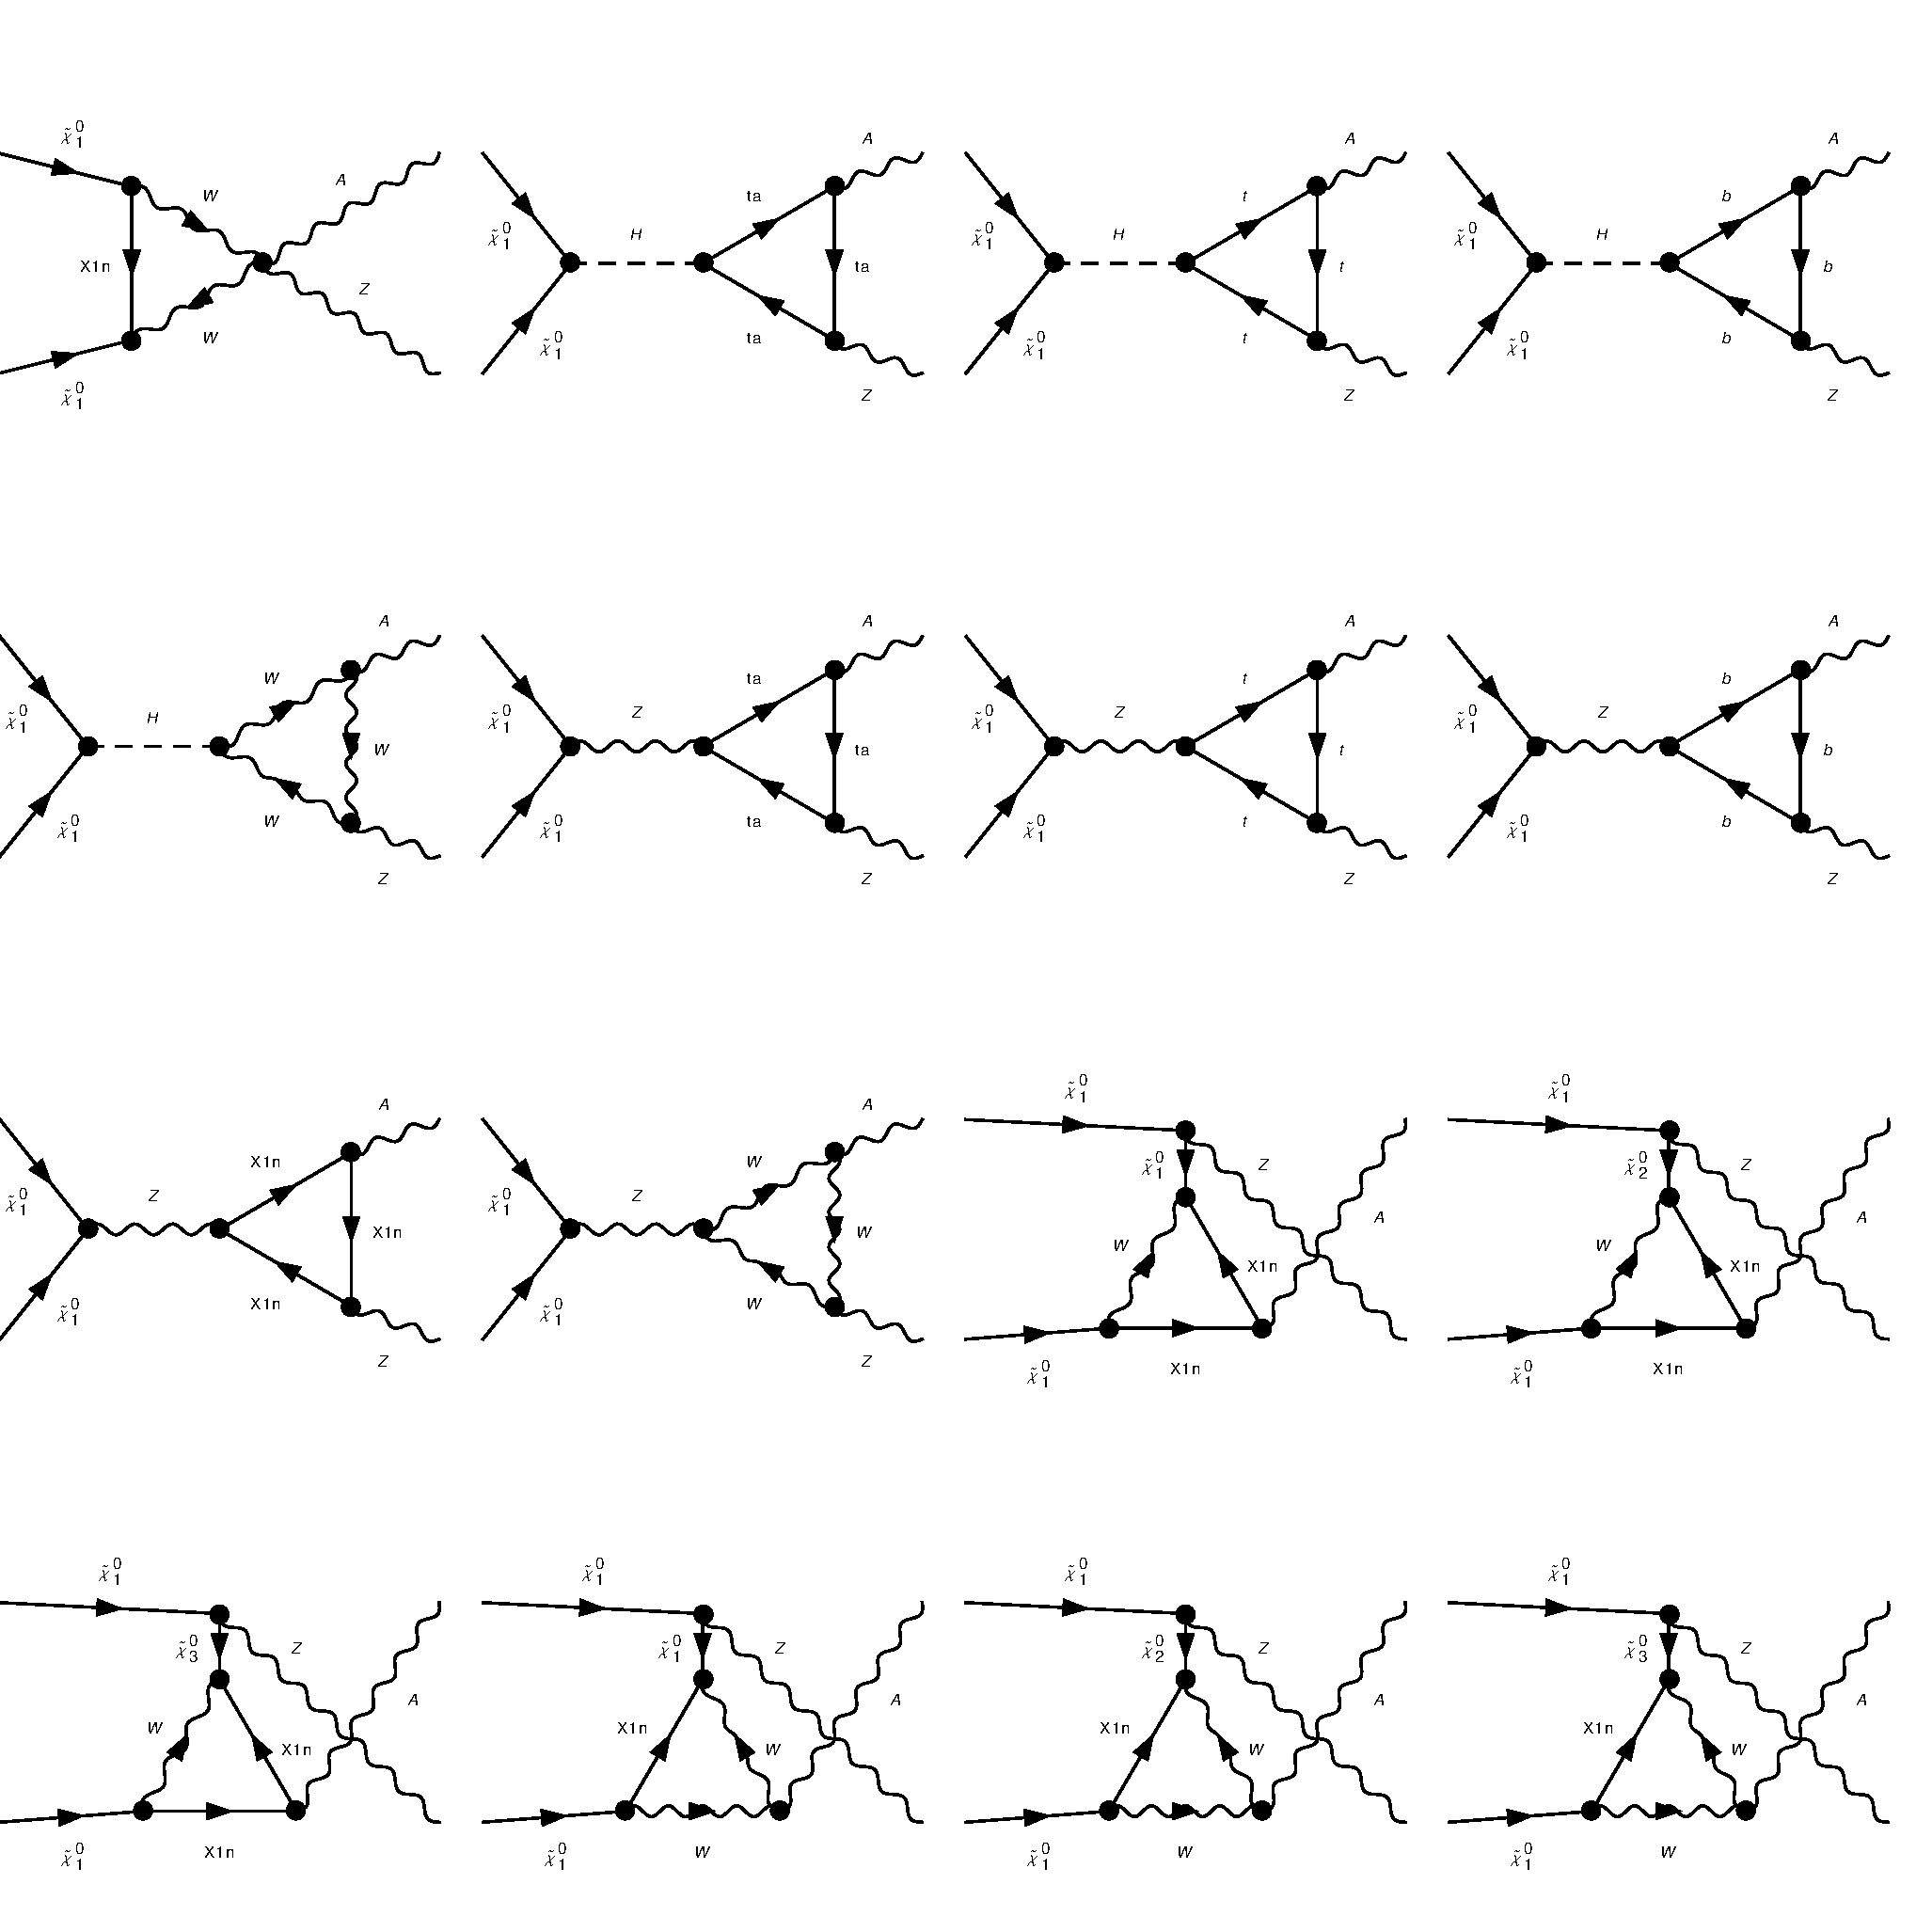
\includegraphics[scale=0.46]{gz1}
%\end{figure}
%%
%\begin{figure}
%\centering
%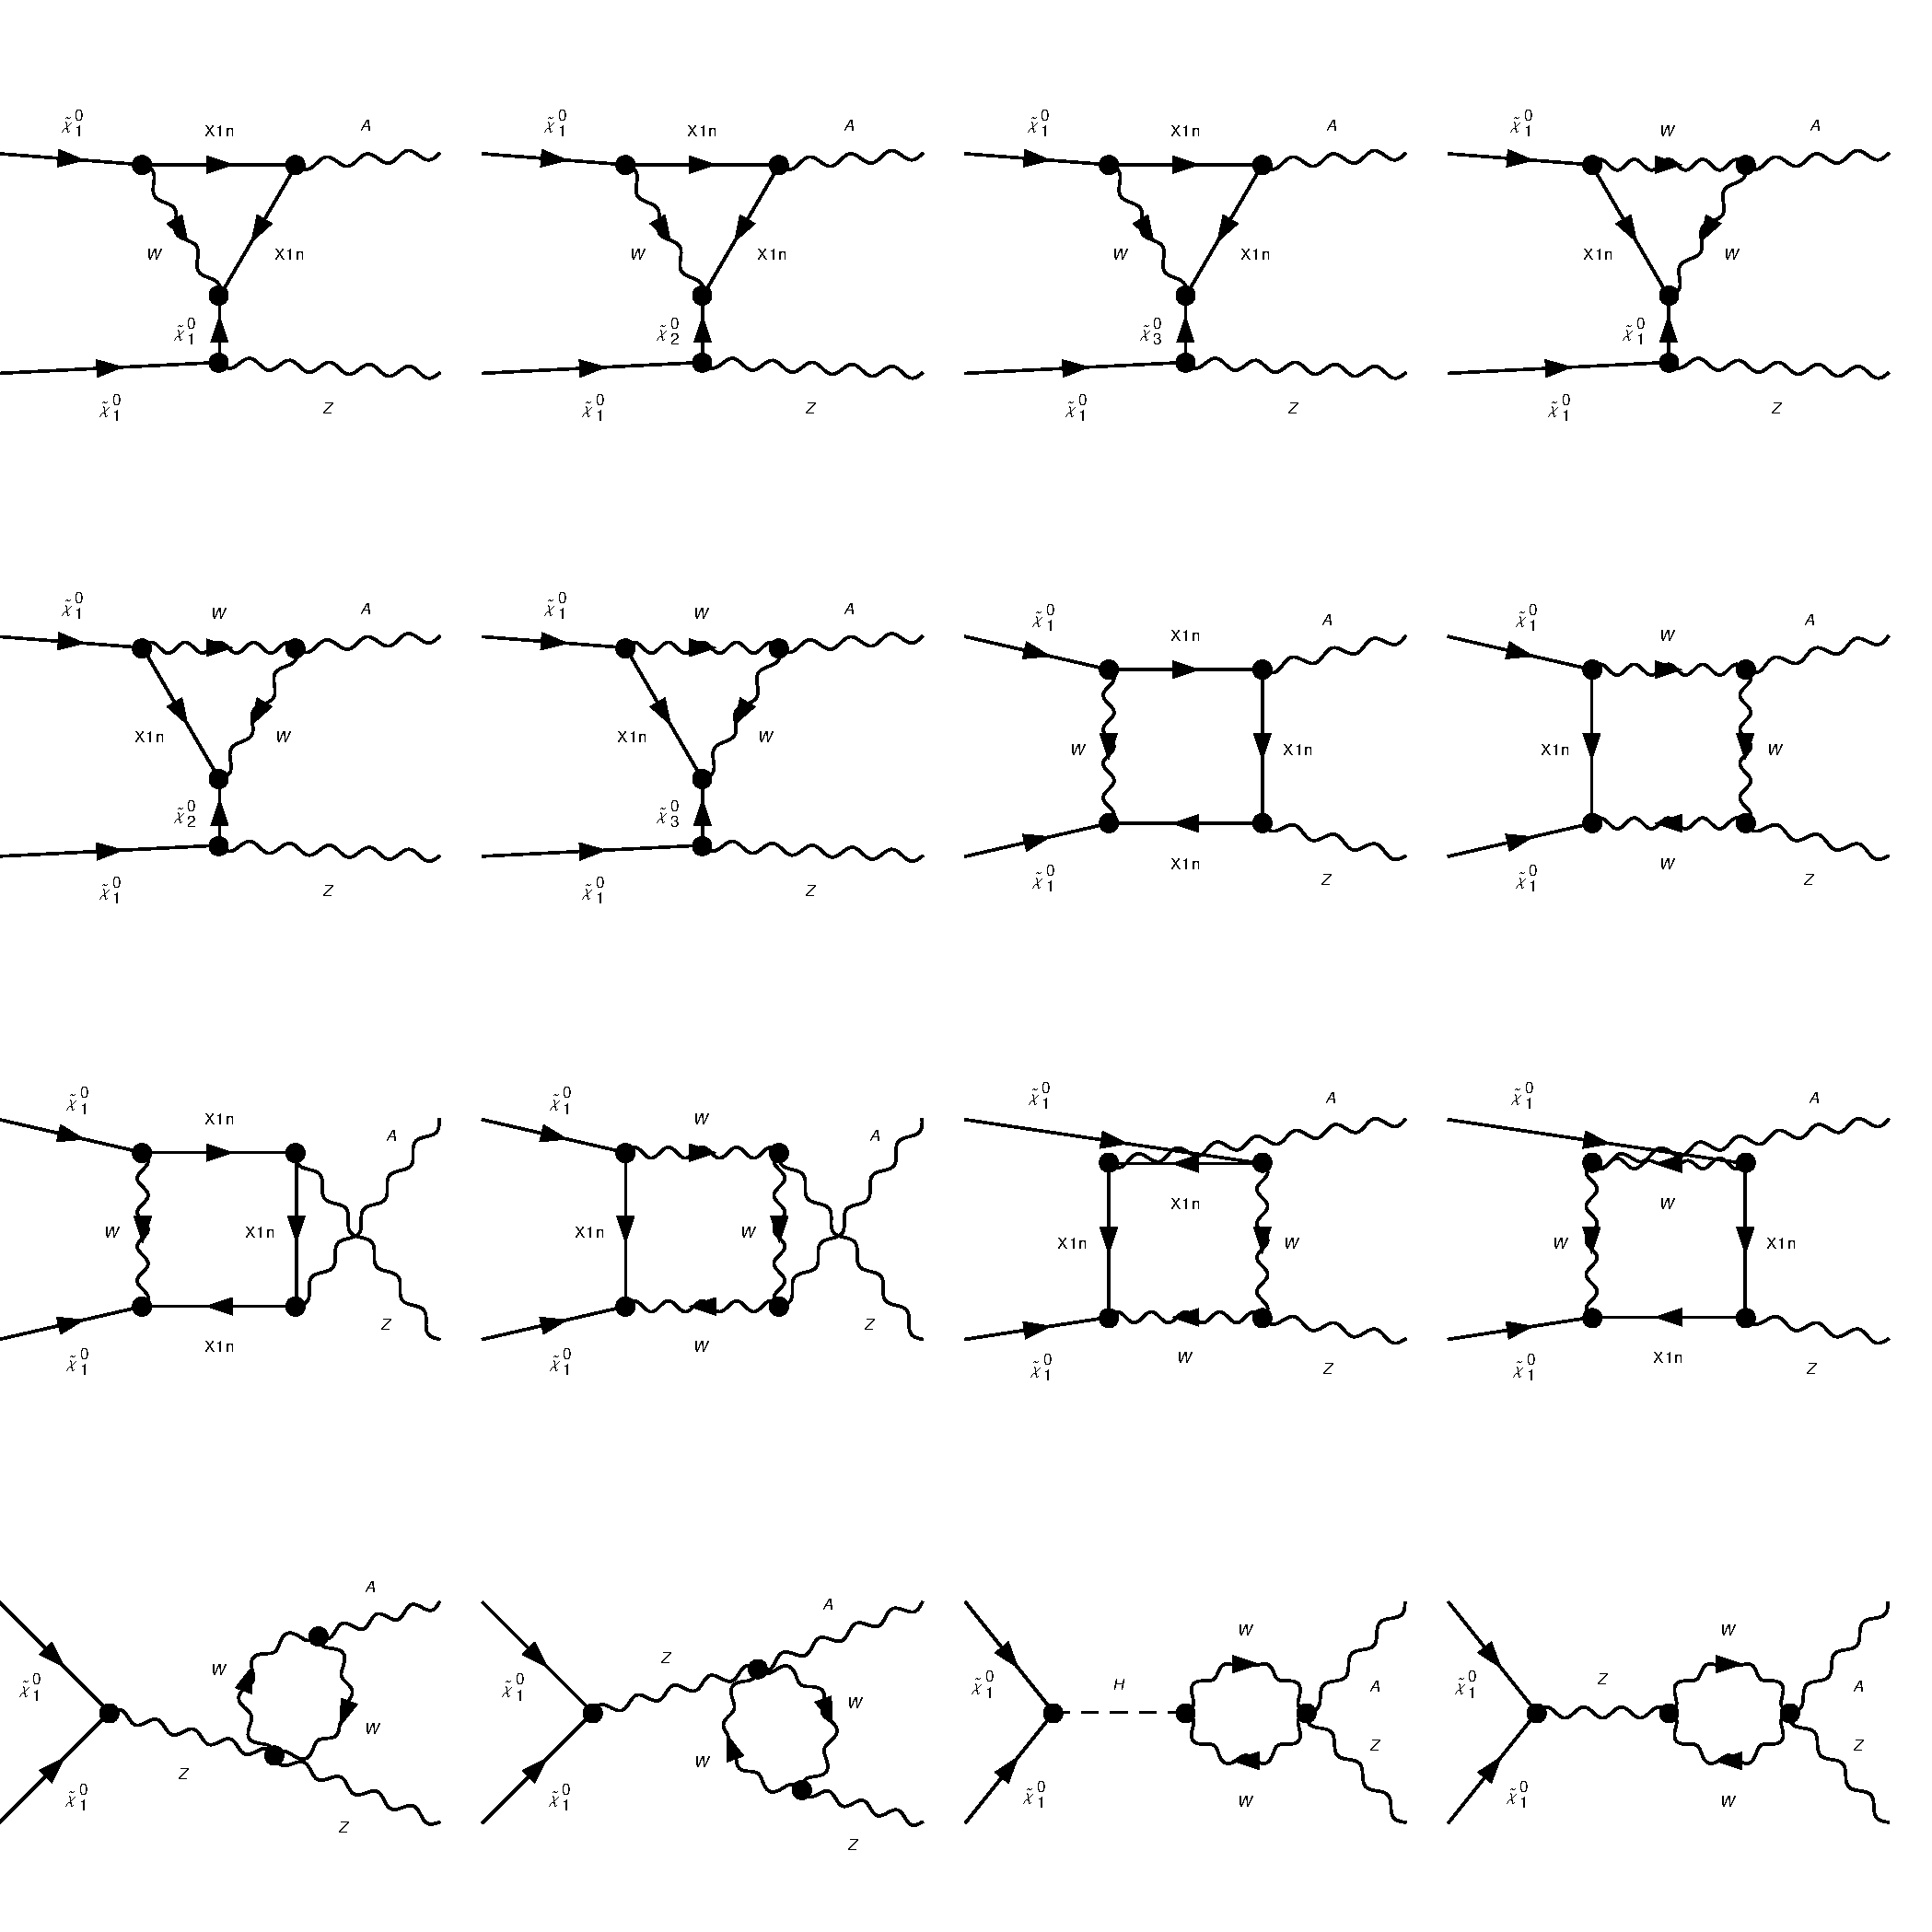
\includegraphics[scale=0.46]{gz2}
%\caption{Feynman diagrams for annihilation into $\gamma Z$ in unitary gauge.}
%\end{figure}
%%